\DocumentMetadata{%
 %  uncompress, %only for debugging!!
  pdfversion=2.0,
  testphase={phase-II, tabular, graphic}%
 % testphase={phase-II,math, tabular, graphic}% TOC Does not work
   % testphase={phase-III,math}% TOC works
}
\tagpdfsetup{activate, tabsorder=structure}
% Use the following to fix bug in November 2023 download of LaTeX
\ExplSyntaxOn
\cs_generate_variant:Nn\__tag_prop_gput:Nnn{cnx}
\ExplSyntaxOff
\documentclass[11pt,
  english,
  letterpaper,
]{article}
\usepackage{sa4ss}
\usepackage{amsmath,amssymb,array}
\usepackage{booktabs}

% From tagged-template.latex
\usepackage{lmodern}
\usepackage{ifxetex,ifluatex}
\ifnum 0\ifxetex 1\fi\ifluatex 1\fi=0 % if pdftex
  \usepackage[T1]{fontenc}
  \usepackage[utf8]{inputenc}
  \usepackage{textcomp} % provide euro and other symbols
\else % if luatex or xetex
  \usepackage{unicode-math}
  \defaultfontfeatures{Scale=MatchLowercase}
  \defaultfontfeatures[\rmfamily]{Ligatures=TeX,Scale=1}
\fi

% Use upquote if available, for straight quotes in verbatim environments
\IfFileExists{upquote.sty}{\usepackage{upquote}}{}
\IfFileExists{microtype.sty}{% use microtype if available
  \usepackage[]{microtype}
  \UseMicrotypeSet[protrusion]{basicmath} % disable protrusion for tt fonts
}{}
\makeatletter
\@ifundefined{KOMAClassName}{% if non-KOMA class
  \IfFileExists{parskip.sty}{%
    \usepackage{parskip}
  }{% else
    \setlength{\parindent}{0pt}
    \setlength{\parskip}{6pt plus 2pt minus 1pt}}
}{% if KOMA class
  \KOMAoptions{parskip=half}}
\makeatother
\usepackage{xcolor}
\IfFileExists{xurl.sty}{\usepackage{xurl}}{} % add URL line breaks if available
\hypersetup{
  pdflang={en},
  hidelinks,
  pdfcreator={LaTeX via pandoc}}
\urlstyle{same} % disable monospaced font for URLs
\usepackage{longtable}
% Correct order of tables after \paragraph or \subparagraph
\usepackage{etoolbox}
\makeatletter
\patchcmd\longtable{\par}{\if@noskipsec\mbox{}\fi\par}{}{}
\makeatother
% Allow footnotes in longtable head/foot
\IfFileExists{footnotehyper.sty}{\usepackage{footnotehyper}}{\usepackage{footnote}}
\makesavenoteenv{longtable}
\usepackage{graphicx}
\makeatletter
\def\maxwidth{\ifdim\Gin@nat@width>\linewidth\linewidth\else\Gin@nat@width\fi}
\def\maxheight{\ifdim\Gin@nat@height>\textheight\textheight\else\Gin@nat@height\fi}
\makeatother
% Scale images if necessary, so that they will not overflow the page
% margins by default, and it is still possible to overwrite the defaults
% using explicit options in \includegraphics[width, height, ...]{}
\setkeys{Gin}{width=\maxwidth,height=\maxheight,keepaspectratio}
% Set default figure placement to htbp
\makeatletter
\def\fps@figure{htbp}
\makeatother
\setlength{\emergencystretch}{3em} % prevent overfull lines
\providecommand{\tightlist}{%
  \setlength{\itemsep}{0pt}\setlength{\parskip}{0pt}}
\setcounter{secnumdepth}{5}
\usepackage{lineno}
\usepackage[inline]{showlabels}
\ifxetex
  % Load polyglossia as late as possible: uses bidi with RTL langages (e.g. Hebrew, Arabic)
  \usepackage{polyglossia}
  \setmainlanguage[]{}
\else
  \usepackage[shorthands=off,main=english]{babel}
\fi

%Define cslreferences environment, required by pandoc 2.8
%https://github.com/rstudio/rmarkdown/issues/1649
\newlength{\csllabelwidth}
\setlength{\csllabelwidth}{3em}
\newlength{\cslhangindent}
\setlength{\cslhangindent}{1.5em}
% for Pandoc 2.8 to 2.10.1
\newenvironment{cslreferences}%
  {}%
  {\par}
% For Pandoc 2.11+
\newenvironment{CSLReferences}[2] % #1 hanging-ident, #2 entry spacing
 {% don't indent paragraphs
  \setlength{\parindent}{0pt}
  % turn on hanging indent if param 1 is 1
  \ifodd #1 \everypar{\setlength{\hangindent}{\cslhangindent}}\ignorespaces\fi
  % set entry spacing
  \ifnum #2 > 0
  \setlength{\parskip}{#2\baselineskip}
  \fi
 }%
 {}
\usepackage{calc}  % for \widthof, \maxof in minipage
\newcommand{\CSLBlock}[1]{#1\hfill\break}
\newcommand{\CSLLeftMargin}[1]{\parbox[t]{\csllabelwidth}{#1}}
\newcommand{\CSLRightInline}[1]{\parbox[t]{\linewidth - \csllabelwidth}{#1}\break}
\newcommand{\CSLIndent}[1]{\hspace{\cslhangindent}#1}


\providecommand{\tightlist}{%
  \setlength{\itemsep}{0pt}\setlength{\parskip}{0pt}}

\usepackage{lineno}
\usepackage[inline]{showlabels}
\date{}
\newcommand{\trTitle}{}
\newcommand{\trYear}{2023}
\newcommand{\trMonth}{May}
\newcommand{\trAuthsLong}{truetruetrue}
\newcommand{\trAuthsBack}{Wetzel, C.R., M.H. Monk, J. Coates}
\newcommand{\trCitation}{
\begin{hangparas}{1em}{1}
\trAuthsBack{}. \trYear{}. \trTitle{}. \glsentrylong{pfmc}, Portland, Oregon. \pageref{LastPage}{}\,p.
\end{hangparas}}

\newcommand\includegraphicsifexists[2][width=\linewidth]{\IfFileExists{#2}{\includegraphics[#1]{#2}}{}}

\begin{document}

%%%%% Frontmatter %%%%%

% Footnote symbols in front matter
\renewcommand*{\thefootnote}{\fnsymbol{footnote}}

\small
\thispagestyle{empty}
\pagenumbering{roman}
\noindent
\begin{center}
\title{}
% \textnormal{\MakeTextUppercase{\trTitle{}}}
\vspace{1.5cm}
{\Large\textbf\newline{}}

\includegraphicsifexists[width=4in]{figure_title.png}
\vfill
by\\
Chantel R. Wetzel\textsuperscript{1}\\
Melissa H. Monk\textsuperscript{2}\\
Julia Coates\textsuperscript{3}\vfill
\textsuperscript{1}Northwest Fisheries Science Center, U.S. Department of Commerce, National Oceanic and Atmospheric Administration, National Marine Fisheries Service, 2725 Montlake Boulevard East, Seattle, Washington 98112\\
\textsuperscript{2}Southwest Fisheries Science Center, U.S. Department of Commerce, National Oceanic and Atmospheric Administration, National Marine Fisheries Service, 110 McAllister Way, Santa Cruz, California 95060\\
\textsuperscript{3}.na.character\vfill
\trMonth{} \trYear{}
\end{center}
\clearpage

% Fourth page: Colophon
\thispagestyle{empty}
\vspace*{\fill}
\begin{center}
\copyright{} \glsentrylong{pfmc}, \trYear{}\\
\end{center}
\par
\bigskip
\noindent
Correct citation for this publication:
\bigskip
\par
\trCitation{}
\clearpage

% Add TOC to pdf bookmarks (clickable pdf)
\pdfbookmark[1]{\contentsname}{toc}

% Table of contents page, lists of figures and tables
\tableofcontents\clearpage
\label{TRlastRoman}
\clearpage

% Table of contents
\newpage
\thispagestyle{empty} % to remove page number

% Settings for the main document
\pagenumbering{arabic}  % Regular page numbers
\pagestyle{plain}  % No page number on first page of main document, use 'empty'
\renewcommand*{\thefootnote}{\arabic{footnote}}  % Back to numeric footnotes
\setcounter{footnote}{0}  % And start at 1
\renewcommand{\headrulewidth}{0.5pt}
\renewcommand{\footrulewidth}{0.5pt}
%\pagestyle{fancy}\fancyhead[c]{Draft: Do not cite or circulate}

\newcommand{\lt}{\ensuremath <}
\newcommand{\gt}{\ensuremath >}

\linenumbers

\newcommand\CapeM{$40^\circ 10^\prime N$}
\newcommand\PtC{$34^\circ 27^\prime N$}
\newcommand\CAOR{$42^\circ 00^\prime N$}

\hypertarget{introduction}{%
\section{Introduction}\label{introduction}}

This assessment report describes the sub-area population of copper rockfish (\emph{Sebastes caurinus}) off the California coast south of Point Conception in U.S. waters, using data through 2022. The sub-area population north of Point Conception in California waters was also evaluated and is described in a separate assessment report. The copper rockfish status for the California stock of is determined by the combined estimates of spawning output from both sub-areas and is detailed in the \protect\hyperlink{management}{Management} section. This assessment does not account for populations located in Mexico waters or other areas off the U.S. coast and assumes that these southern and northern populations do not contribute to the population being assessed here.

\hypertarget{basic-information-and-life-history}{%
\subsection{Basic Information and Life History}\label{basic-information-and-life-history}}

Copper rockfish have historically been a part of both commercial and recreational fisheries throughout its range. Copper rockfish are a demersal, relatively nearshore species within the subgenus \emph{Pteropodus.} The copper rockfish's core range is c omparatively large, ranging from northern Baja Mexico to the Gulf of Alaska, with copper rockfish also found in Puget Sound. Copper rockfish range from the subtidal (as juveniles) to depths of 183 m (Love et al. 2002). Copper rockfish are commonly found in waters less than 100 meters in depth inhabiting nearshore kelp forests and complex low-relief rocky habitat (Love 1996). Adult copper rockfish have high site fidelity and do not make long-range movements. An acoustic telemetry study displaced copper rockfish 4km from their capture location to an artificial reef and within 10 days, half of the copper rockfish returned to the original capture location (Reynolds et al. 2010).

Copper rockfish have a clearly defined long white band the posterior two-thirds of the lateral line. Copper rockfish has high variation in coloration throughout its range, taking on coloration from dark brown, olive, orange-red and pink, with patches of yellow and pink (Miller and Lea 1972). In general the copper rockfish towards the northern part of the range are often darker in color than fish encountered in southern California. The distinct change in coloration resulted in copper rockfish described as two separate species, copper rockfish (\emph{S. caurinus}) and whitebelly rockfish (\emph{S. vexillaris}).

The \emph{Sebastes} genus are viviparous with internal fertilization, many exhibit dimorphic growth with females larger at size-at-age than males, and a number of species have reproductive strategies that vary with latitude. There are very few fecundity samples from copper rockfish available from available from California, although copper rockfish are assumed to produce a single brood annually during the winter months.

The pelagic larvae are encountered in the CalCOFI surveys, but neither larval nor young-of-the-year (YOY) can be identified copper rockfish visually (Thompson et al. 2017). The size at birth ranges from 5-6 mm and the larvae remain pelagic until approximately 22-23 mm standard length at which time they recruit to the kelp forest canopy (Anderson 1983).

Juvenile Copper rockfish are indistinguishable from kelp (\emph{S. atrovirens}), black-and-yellow (\emph{S. chrysomelas}), and gopher rockfish (\emph{S. carnatus}), all of which recruit to the kelp forest canopy in the spring months. Copper rockfish is the first of the species group to recruit to the kelp forest from April to May and can be distinguished from the other species once it reaches a size around 50 mm standard length (Anderson 1983). Baetscher genetically identified YOY rockfish from surveys in Carmel and Monterey Bays in California and provided the authors with the length and genotyped species idenifications from her study (Baetscher et al. 2019). The average length of copper rockfish in July was 3-4 cm total length \ref{fig:copper-smurf-length}. Anderson observed benthic copper rockfish nocturnally active over sandy bottom outside the kelp forest (Anderson 1983).

Copper rockfish are a relatively long-lived rockfish, estimated to live at least 50 years (Love 1996). Copper rockfish was determined to have the highest vulnerability (V = 2.27) of any West Coast groundfish stock evaluated in a productivity susceptibility analysis (Cope et al. 2011). This analysis calculated species-specific vulnerability scores based on two dimensions: productivity characterized by the life history and susceptibility that characterized how the stock could be impacted by fisheries and other activities.

As adults, there is little evidence of movement, with Hanan and CCFRP citations

Copper rockfish are opportunistic carnivores and commonly consume crustaceans, mollusks, and fish whole (Lea et al. 1999; Bizzarro et al. 2017). (1972) observed a shift in a diet dominated by arthropods in age 0 and 1 fish, and a shift to a more diverse diet including molluscs and fish as they aged. the study also noted that juvenile copper rockfish were predated on by harbor seals and lingcod.

There is currently no evidence of significant stock structure from genetic studies of copper rockfish across the west coast. (2002) looked at genetic variation across six micosatellite DNA loci from samples ranging from British Columbia to southern California. Significant population subdivision was detected between th Puget Sound and coastal samples and support the model of isolation-by-distance for copper rockfish. Sivasundar and Palumbi (2010) conducted a genetic study to determine the potential for biogeographic boundaries to prohibit gene flow for 15 \emph{Sebastes} species. The study's sample sizes of copper rockfish with samples form Oregon, Monterey Bay and Santa Barbara. Sivasundar and Palumbi (2010) used mtDNA and could differentiate samples from Santa Barbara from those collected in Oregon and Monterey Bay, but the Monterey Bay and Oregon samples could not be distinguished. Micosatellite data did not reveal any genetic differentiation among the sampels from the three locations for copper rockfish and suggests low genetic differentiation coastwide.

The most recent genetic analysis of copper rockfish to date was conducted by Johansson et al. (2008). The study included 749 samples from along the west coast ranging from Neah Bay, Washington to San Diego, California with the majority of sampling locations clustered north of Cape Mendocino in northern California. The study included 185 samples collected within California. Eleven microsatellite DNA loci were analyzed. The study found significant evidence to support isolation by distance at the coast wide scale. Weak, but significant, genetic structure was identified from samples collected along the Oregon coast suggesting that habitat barriers may limit larval dispersal.

\hypertarget{ecosystem-considerations}{%
\subsection{Ecosystem Considerations}\label{ecosystem-considerations}}

This stock assessment does not explicitly incorporate trophic interactions, habitat factors (other than as they inform relative abundance indices) or environmental factors into the assessment model, but a brief description of likely or potential ecosystem considerations are provided below.

As with most other rockfish and groundfish in the California Current, recruitment, or cohort (year-class) strength appears to be highly variable for the copper rockfish complex, with only a modest apparent relationship to estimated levels of spawning output. Oceanographic and ecosystem factors are widely recognized to be key drivers of recruitment variability for most species of groundfish, as well as most elements of California Current food webs. Empirical estimates of recruitment from pelagic juvenile rockfish surveys have been used to inform incoming year class strength for some of these stocks, however copper rockfish are infrequently encountered in these surveys. Between 1998 and 2013 the California Cooperative Oceanic Fisheries Investigation (CalCOFI) survey observed had 34 positive observations copper rockfish out of nearly 300,000 total juvenile \emph{Sebastes} encountered in juvenile surveys.

\hypertarget{historical-and-current-fishery-information}{%
\subsection{Historical and Current Fishery Information}\label{historical-and-current-fishery-information}}

Off the coast of California south of Point Conception copper rockfish is caught in both commercial and recreational fisheries. Recreational removals have been the largest source of fishing mortality of copper rockfish across all years (Table \ref{tab:allcatches} and Figure \ref{fig:catch}). The recreational fishery is comprised of individual recreational fishers (Private/Rental, PR) and charter recreational private vessels (CPFV) which take groups of individuals out for day fishing trips. Across both types of recreational fishing the majority of effort occurs around rocky reefs that can be accessed via a day-trips.

The recreational fishery in the early part of the 20th century was focused on nearshore waters near ports, with expanded activity further from port and into deeper depths over time (Miller et al. 2014). Prior to the groundfish fishery being declared a federal disaster in 2000, and the subsequent rebuilding period, there were no time or area closures for groundfish. Access to deeper depths during this period spread effort over a larger area and filled bag limits with a greater diversity of species from both the shelf and nearshore. This resulted in lower catch of nearshore rockfish relative to the period after 2000 when 20 to 60 fm depth restrictions ranging from 20 fm in the Northern Management Area to 60 fm in the Southern Management Area were put in place in various management area delineations along the state. This shifting effort onto the nearshore, concomitantly increased catch rates for nearshore rockfish including copper rockfish in the remaining open depths, though season lengths were greatly curtailed.

Following all previously overfished groundfish species, other than yelloweye rockfish, being declared rebuilt by 2019, deeper depth restrictions were offered in the Southern Management area allowing resumed access to shelf rockfish in less than 75 fm and are currently 100 fm as of 2021. The increased access to deeper depths south of Point Conception with the rebuilding of cowcod is expected to reduce the effort in nearshore waters where copper rockfish is most prevalent. To the north of Point Conception where yelloweye rockfish are prevalent, depth constraints persist and effort remains focused on the nearshore in 30 to 50 fm depending on the management area. As yelloweye rockfish continues to rebuild, incremental increases in access to deeper depths are expected, which will likely further reduce the effort in nearshore waters where copper rockfish is most prevalent.

Prior to development of the live fish market in the 1980s, there was very little commercial catch of copper rockfish, with dead copper rockfish fetching a low ex-vessel price per pound. Copper rockfish were targeted along with other rockfish to some degree in the nearshore or caught as incidental catch by vessels targeting other more valuable stocks such as lingcod. Most fish were caught using hook and line gear, though some were caught using traps, gill nets and, rarely, trawl gear. Trawling was prohibited within three miles of shore in 1953 and gill netting within three miles of shore was prohibited in 1994, preventing access to a high proportion of the species habitat with these gear types. Copper rockfish were caught along with other rockfish to some degree in the nearshore or caught as bycatch by vessels targeting other more valuable stocks such as lingcod.

In the late 1980s and early 1990s a market for fish landed live arose out of Los Angeles and the Bay area, driven by demand from Asian restaurants and markets. The growth of the live fish market was driven by consumers willing to pay a higher price for live fish, ideally plate-sized (12 - 14 inches or 30.5 - 35.6 cm). Live fish landed for the restaurant market are lumped into two categories, small (1 - 3 lbs.) or large (3 - 6 lbs.), with small, plate-sized, fish fetching higher prices at market ranging between \$5 -7 per fish (Bill James, personal communication). Copper rockfish is one of the many rockfish species that is included in the commercial live fish fishery. The proportion of copper rockfish being landed live vs.~dead since 2000 by California commercial fleets ranges between 50 to greater than 70 percent in the southern and northern areas, respectively.

With the development and expansion of the nearshore live fish fishery during the 1980s and 1990s, new entrants in this open access fishery were drawn by premium ex-vessel price per pound for live fish, resulting in over-capitalization of the fishery. Since 2002, the California Department of Fish and Wildlife (CDFW) has managed 19 nearshore species in accordance with Nearshore Fisheries Management Plan (Wilson-Vandenberg et al. 2014). In 2003, the CDFW implemented a Nearshore Restricted Access Permit system, including the requirement of a Deeper Nearshore Fishery Species Permit to retain copper rockfish, with the overall goal of reducing the number of participants to a more sustainable level, with permit issuance based on historical landings history by the retrospective qualifying date. The result was a reduction in permits issued from 1,127 in 1999 to 505 in 2003, greatly reducing catch levels. In addition, reduced trip limits, season closures in March and April and depth restrictions were implemented to address bycatch of overfished species and associated constraints from their low catch limits.

Copper rockfish residing between Point Conception and the California/Oregon border are assessed here as a single, separate stock (Figure \ref{fig:ca-map}). This designation was made based on oceanographic, geographic, and fishery conditions. The copper rockfish population in California waters was split at Point Conception due to water circulation patterns that create a natural barrier between nearshore rockfish populations to the north and south. The northern border for this assessment was defined as the California/Oregon border due to substantial differences in historical and current exploitation levels. Additionally, the fairly sedentary nature of adult copper rockfish, likely limits flow of fish between northern California and areas to the north.

\hypertarget{summary-of-management-history-and-performance}{%
\subsection{Summary of Management History and Performance}\label{summary-of-management-history-and-performance}}

Prior to the adoption of the Pacific Coast Groundfish Fishery Management Plan (FMP) in 1982, copper rockfish were managed through a regulatory process that included the California Department of Fish and Wildlife (CDFW), the California State Legislature, and the Fish and Game Commission (FGC). With implementation of the Pacific Coast Groundfish FMP, copper rockfish came under the management authority of the Pacific Fishery Management Council (PFMC) and were managed as part of the Sebastes complex. Because copper rockfish had not undergone rigorous stock assessment and did not compose a large fraction of the landings it was classified and managed as part of the ``Minor Nearshore Rockfish'' group (PFMC 2008).

Since the early 1980s, a number of federal regulatory measures have been used to manage the commercial rockfish fishery including cumulative trip limits (generally for two- month periods) and seasons. Starting in 1994 the commercial groundfish fishery sector was divided into two components: limited entry and open access with specific regulations designed for each component. Limited entry programs were designed in part to limit bottom contact gears and the open access sector includes gears not making bottom contact, e.g.~hook and line. Other regulatory actions for the general rockfish categories included area closures and gear restrictions set for the four different commercial sectors - limited entry fixed gear, limited entry trawl, open access trawl, and open access non-trawl (which includes the nearshore fishery) .

During the late 1990s and early 2000s, major changes also occurred in the way that California managed its nearshore fishery. The Marine Life Management Act (MLMA), which was passed in 1998 by the California Legislature and enacted in 1999, required that the FGC adopt an FMP for nearshore finfish (Wilson-Vandenberg et al.~2014). It also gave authority to the FGC to regulate commercial and recreational nearshore fisheries through FMPs and provided broad authority to adopt regulations for the nearshore fishery during the time prior to adoption of the nearshore finfish FMP. Within this legislation, the Legislature also included a requirement that commercial fishermen landing nearshore species possess a nearshore fishery permit. In 2000, the PFMC's rockfish management structure changed significantly with the replacement of the Sebastes complex -north and -south areas with Minor Rockfish North (Vancouver, Columbia, and Eureka, International North Pacific Fisheries Commission (INPFC) areas) and Minor Rockfish South (Monterey and Conception INPFC areas only). The OY for these two groups was further divided (between north and south of 40\(^\circ\) 10' N. lat., Cape Mendocino, California) into nearshore, shelf, and slope rockfish categories with allocations set for Limited Entry and Open Access fisheries within each of these three categories (January 4, 2000, 65 FR 221; PFMC 2002, Tables 54-55). Species were parceled into these new categories depending on primary catch depths and geographical distribution. copper rockfish was included in the nearshore rockfish category.

Following adoption of the Nearshore FMP and accompanying regulations by the FGC in fall of 2002, the FGC adopted regulations in November 2002 which established a set of marine protected areas (MPAs) around the Channel Islands in southern California (which became effective April 2003). The FGC also adopted a restricted access program in December 2002 which established the Deeper Nearshore Species Fishery Permit, to be effective starting in the 2003 fishing year. Also, since the enactment of the MLMA, the PFMC and State coordinated to develop and adopt various management specifications to keep harvest within the harvest targets, including seasonal and area closures, depth restrictions, and bag limits to regulate the recreational fishery and license and permit regulations, finfish trap permits, gear restrictions, seasonal and area closures, depth restrictions, trip limits, and minimum size limits to regulate the commercial fishery. The MPAs were later expanded under authority of the Marine Life Protection Act (MLPA) enacted in 1999, creating a network of MPAs which went into place in phases beginning with the central coast in 2007, north central coast in 2010, and the south and north coasts in 2012. The implementation of the cowcod conservation area (CCA) in 2001 closed a large area of the Southern California Bight west of Santa Catalina and San Clemente Islands and offshore of San Diego. The CCA prohibited retention of groundfish, except for some take of nearshore species in depths less than 20 fm around islands and banks, and later, less than 40 fm. The rockfish conservation areas (RCAs) are seasonally adjusted depth limits impacting trawl and non-trawl gears that were initially established in 2002 to protect overfished species. The RCAs also restricted catch of nearshore species to depths less than 30 fm, and in some areas along California to less than 20 fm. Thus, the MPAs, CCAs and RCAs represent three types of spatial and/or depth closures impacting rockfish.

The state of California has adopted regulatory measures to manage the nearshore fishery based on the harvest guidelines set by the PFMC for the minor nearshore rockfish complexes north and south of 40\(^\circ\) 10' N. lat. The complexes are managed based on overfishing limits (OFL) and annual catch limits (ACL) that are determined by summing the species-specific OFLs and ACLs (ACLs set equal to the Acceptable Biological Catches) contributions for all stocks managed in the complexes). Limits are shared among all commercial and recreational fleets with the various management procedures intended to maintain removals below the total OFL and ACL for the nearshore rockfish north and south complexes as a whole, rather than on a species by species basis. The nearshore commercial fishery is managed based on bimonthly allowable catches per vessel, that have ranged from 200 pounds to 2,000 pounds per two months since 2000. The limited entry trawl fleet is managed on monthly limits on an annual basis. Since 2011, the limit has been 300 pounds per month for non-IFQ species, such as nearshore rockfish.

The species-specific OFL and ACL contribution for copper rockfish that is allocated to California waters, Nearshore Rockfish South and 25 percent of the Nearshore Rockfish North for copper rockfish, is shown in Table \ref{tab:ca-management} as well as the total catch, south and north of Point Conception, of copper rockfish in California for the last ten years. Over the last ten years the catches of copper rockfish have been below the species-specific ACLs. In 2021 all West Coast stocks of copper rockfish were assessed that informed the 2023-24 harvest specifications OFLs and ACLs for copper rockfish. In California waters the new OFLs and ACLs for the 2023-24 management cycle were significantly lower than early years, resulting in in-season management action by CDFW for 2022 to reduce removals based on the latest stock assessment. January 1, 2022, a statewide commercial sub-trip limit of 75 lbs. per 2-month and statewide recreational sub-bag limit of 1 fish within the overall 10 fish allowed for the RCG complex went into effect. No change in recreational seasons or depth limits occurred in 2022 but changes were implemented in 2023. In 2022, the Northern and Mendocino management areas were closed January through April and allowed fishing to 30 fathoms May through October and at all depths November through December. The San Francisco and Central management areas were closed January through March and allowed fishing to 50 fathoms the remainder of the year. The Southern management area was closed January and February and allowed fishing to 100 fathoms the remainder of the year. Beginning in 2023, closed seasons are extended in all management areas. Depth restrictions are eased during some months and tightened in others.

\hypertarget{foreign-fisheries}{%
\subsection{Foreign Fisheries}\label{foreign-fisheries}}

\emph{Sebastes} spp. are not in the Fisheries National Chart (FNC, database containing species status) maintained by the Mexican Government, i.e., they are not commercially harvested in the northwest Mexican Pacific Ocean (E.M. Bojórquez, Centro de Investigaciones Biológicas del Noroeste, S.C., personal communication).There are no data available on copper rockfish fisheries off the coast of Mexico. Catches in Mexican waters by U.S. fleets are not included in this assessment.

\hypertarget{data}{%
\section{Data}\label{data}}

Data comprise the foundational components of stock assessment models. The decision to include or exclude particular data sources in an assessment model depends on many factors. These factors often include, but are not limited to, the way in which data were collected (e.g., measurement method and consistency); the spatial and temporal coverage of the data; the quantity of data available per desired sampling unit; the representativeness of the data to inform the modeled processes of importance; timing of when the data were provided; limitations imposed by the Pacific Fishery Management Council Groundfish Terms of Reference; and the presence of an avenue for the inclusion of the data in the assessment model. Attributes associated with a data source can change through time, as can the applicability of the data source when different modeling approaches are explored (e.g., stock structure or time-varying processes). Therefore, the specific data sources included or excluded from this assessment should not necessarily constrain the selection of data sources applicable to future stock assessments for copper rockfish. Even if a data source is not directly used in the stock assessment they can provide valuable insights into biology, fishery behavior, or localized dynamics.

Data from a wide range of programs were available for possible inclusion in the current assessment model. Descriptions of each data source included in the model (Figure \ref{fig:data-plot}) and sources that were explored but not included in the base model are provided below. Data that were excluded from the base model were explicitly explored during the development of this stock assessment or have not changed since their past exploration in a previous copper rockfish stock assessment. In some cases, the inclusion of excluded data sources were explored through sensitivity analyses (see Section \ref{assessment-model}).

\hypertarget{biological-data}{%
\subsection{Biological Data}\label{biological-data}}

\hypertarget{natural-mortality}{%
\subsubsection{Natural Mortality}\label{natural-mortality}}

Natural mortality was not directly measured, so life-history based empirical relationships were used. The Natural Mortality Tool (NMT), a Shiny-based graphical user interface allowing for the application of a variety of natural mortality estimators based on measures such as longevity, size, age and growth, and maturity, was used to obtain estimates of natural mortality. The NMT currently provides 19 options, including the Hamel (2022) method, which is a corrected form of the Then et al. (2015) functional regression model and is a commonly applied method for West Coast groundfish. The NMT also allows for the construction of a natural mortality prior weighted across methods by the user.

The Hamel (2022) method for developing a prior on natural mortality for West Coast groundfish stock assessments combines meta-analytic approaches relating the \(M\) rate to other life-history parameters such as longevity, size, growth rate, and reproductive effort to provide a prior for \(M\). The Hamel (2022) method re-evaluated the data used by Then et al. (2015) by fitting the one-parameter \(A_{\text{max}}\) model under a log-log transformation (such that the slope is forced to be -1 in the transformed space (Hamel 2015), the point estimate and median of the prior for \(M\) is:

\begin{centering}

$M=\frac{5.4}{A_{\text{max}}}$

\end{centering}

\vspace{0.5cm}

where \(A_{\text{max}}\) is the maximum age. The prior is defined as a lognormal distribution with mean \(ln(5.4/A_{\text{max}})\) and standard error = 0.31. Using a maximum age of 50, the point estimate and median of the prior is 0.108 yr\textsuperscript{-1}. The maximum age was selected based on available age data from all West Coast data sources and literature values. The oldest aged copper rockfish observed in California waters was 52 years of age sampled in 2020 in northern California with 15 additional fish aged to be 40 years and older across all data sources.

The maximum age in the model was set at 50 years. This selection was consistent with the literature examining the longevity of copper rockfish within California (Love 1996) and was supported by the observed ages that had multiple observations of fish between 40 and 52 years of age.

\hypertarget{maturation-and-fecundity}{%
\subsubsection{Maturation and Fecundity}\label{maturation-and-fecundity}}

Maturity-at-length was based on maturity reads conducted by Melissa Head at the NWFSC examining a total of 112 samples (18 north of Point Conception and 94 south of Point Conception) collected across California by the NWFSC Hook and Line survey and the NWFSC WCGBT surveys collected in September and October. Given the limited sample size north of Point Conception, all samples were pooled across California to inform maturity north of Point Conception, while only samples south of Point Conception were used to inform maturity in this region.

The maturity-at-length curve is based on an estimate of functional maturity rather than biological maturity. Biological maturity can include multiple behaviors that functional will exclude (e.g., abortive maturation and skip spawning). Biological maturity indicates that some energy reserves were used to create vitellogenin, but it does not mean that eggs will continue to develop and successfully spawn. This includes juvenile abortive maturation. Female rockfish commonly go through the first stages of spawning the year before they reach actual spawning capability. This is most likely a factor related to their complicated reproductive process of releasing live young. A subset of oocytes will develop early yolk, and then get aborted during the spawning season. Biological maturity also does not account for the proportion of oocytes in atresia (cellular breakdown and reabsorption), which means that fish that were skipping spawning for the season could be listed as biologically mature and functionally immature (Melissa Head, personal communication, NWFSC, NOAA).

The 50 percent size-at-maturity for copper rockfish south of Point Conceptionwas estimated at 34 cm with a slope of -0.41 (Figure \ref{fig:maturity}). This area-specific maturity-at-length estimate is relatively similar but with fish maturing at a slightly smaller size compared to the biological maturity curve assumed for copper rockfish north of Point Conception. Additionally, these values are both slightly smaller compared to estimates by Hannah (2014) for fish observed in Oregon waters (34.8 cm) which estimated the 50 percent size-at-maturity of and slope of -0.60.

The fecundity-at-length was based on research from Dick et al. (2017). The fecundity relationship for copper rockfish was estimated equal to 3.362e-07\(L\)\textsuperscript{3.68} in millions of eggs where \(L\) is length in cm. Fecundity-at-length is shown in Figure \ref{fig:fecundity}.

\hypertarget{sex-ratio}{%
\subsubsection{Sex Ratio}\label{sex-ratio}}

There were limited sex-specific observations by length or age of young fish across biological data sources. The NWFSC WCGBT survey had the highest frequency of small fish observed. However, many of the small fish observed by the survey were too small for sex determination (Figure \ref{fig:frac-sex-len}). In the absence of evidence of a differential sex ratio at birth the sex ratio of young fish was assumed to be 1:1.

\hypertarget{length-weight-relationship}{%
\subsubsection{Length-Weight Relationship}\label{length-weight-relationship}}

The length-weight relationship for copper rockfish was estimated outside the model using all coastwide biological data available from fishery-independent data from the NWFSC WCGBT and the NWFSC Hook and Line surveys. The estimated length-weight relationship for female fish was W = 9.6e-06\(L\)\textsuperscript{3.19} and males 1.11e-05\(L\)\textsuperscript{3.15} where \(L\) is length in cm and W is weight in kilograms (Figure \ref{fig:weight-length}).

\hypertarget{length-at-age}{%
\subsubsection{Growth (Length-at-Age)}\label{length-at-age}}

Length-at-age was estimated for male and female copper rockfish informed by age data from the fisheries, the CCFRP survey, and independent age data collected effort from three programs \texttt{r}area` since 2002: 207 otoliths collected by the NWFSC WCGBT survey, 427 otoliths collected by a research survey conducted by Don Pearson, 77 from a research survey conducted by Abrams, and 508 otoliths collected by a cooperative research survey by the SWFSC and CPFV funded by the Sportfishing Association of California (Table \ref{tab:growth-age-samps}). The ages collected by these three sources were included in the model as a ``growth'' fleet that was not associated with removals or an index of abundance.

Sex-specific growth parameters south of Point Conception were initially estimated external to the model at the following values:

\begin{centering}

Females $L_{\infty}$ = 45.1; $L1$ = 1.13 cm; $k$ = 0.257 per year

Males $L_{\infty}$ = 44.8 cm; $L1$ = 4.75 cm; $k$ = 0.262 per year

\end{centering}

\vspace{0.50cm}

These values were used as starting parameter values within the base model prior to estimating each parameter for male and female copper rockfish.

\hypertarget{ageing-precision-and-bias}{%
\subsubsection{Ageing Precision and Bias}\label{ageing-precision-and-bias}}

Uncertainty surrounding the age-reading error process for copper rockfish was incorporated by estimating ageing error by age. Age composition data used in the model were from break-and-burn otolith reads. Aged copper rockfish used in the assessment were aged by the Cooperative Ageing Project (CAP) in Newport, Oregon. Within-lab ageing error was estimated for CAP based on one primary age reader and a second reader producing double reads from 875 otoliths provided by the CAP lab (Figure \ref{fig:age-error-dist}).

An ageing error estimate was made based on these double reads using a computational tool specifically developed for estimating ageing error (Punt et al. 2008) and using release 1.1.0 of the R package \href{https://github.com/nwfsc-assess/nwfscAgeingError}{nwfscAgeingError} (Thorson et al. 2012) for input and output diagnostics. A linear standard error was estimated by age where there is more variability in the age of older fish (Figures \ref{fig:age-error} and \ref{fig:age-error-matrix}). Sensitivities to alternative ageing error estimates (curvilinear relationship with age) were conducted during model development and the model was relatively insensitive to alternative ageing error assumptions.

\hypertarget{mrfss-index}{%
\section{Appendix B. MRFSS CPFV Dockside Index of Abundance}\label{mrfss-index}}

From 1980 to 2003 the MRFSS program conducted dockside intercept surveys of the recreational CPFV fishing fleet. No MRFSS CPUE data are available for the years 1990-1992, due to a hiatus in sampling related to funding issues. Sampling of California CPFVs north of Point Conception was further delayed, and CPFV samples in 1993 and 1994 are limited to San Luis Obispo County. For purposes of this assessment, the MRFSS time series was truncated at 1999 due to sampling overlap with the onboard observer program (i.e., the same observer samples the catch while onboard the vessel and also conducts the dockside intercept survey for the same vessel).

Each entry in the RecFIN Type 3 database corresponds to a single fish examined by a sampler at a particular survey site. Since only a subset of the catch may be sampled, each record also identifies the total number of that species possessed by the group of anglers being interviewed. The number of anglers and the hours fished are also recorded. The data, as they exist in RecFIN, do not indicate which records belong to the same boat trip. A description of the algorithms and process used to aggregate the RecFIN records to the trip level is outlined in the Supplemental Materials (``Identifying Trips in RecFIN'').

From 1980 to 2003 the MRFSS program conducted dockside intercept surveys of the recreational CPFV fishing fleet. No MRFSS CPUE data are available for the years 1990-1992, due to a hiatus in sampling related to funding issues. Sampling of California CPFVs north of Point Conception was further delayed, and CPFV samples in 1993 and 1994 are limited to San Luis Obispo County. For purposes of this assessment, the MRFSS time series was truncated at 1999 due to sampling overlap with the onboard observer program, i.e., the same observer samples the catch while onboard the vessel and also conducts the dockside intercept survey for the same vessel. The onboard observer data provide higher resolution data of retained and discarded catch.

Each entry in the RecFIN Type 3 database corresponds to a single fish examined by a sampler at a particular survey site. Since only a subset of the catch may be sampled, each record also identifies the total number of that species possessed by the group of anglers being interviewed. The number of anglers and the hours fished are also recorded. The data, as they exist in RecFIN, do not indicate which records belong to the same boat trip. A description of the algorithms and process used to aggregate the RecFIN records to the trip level is outlined in the Supplemental Materials (``Identifying Trips in RecFIN'').

Trips recorded with a primary area fished in Mexico or in bays, e.g., San Francisco Bay, were excluded before any filtering on species composition. For indices representing only north of Point Conception, the years 1993-1994 were excluded due to limited spatial coverage.

The Stephens-MacCall (\textbf{Stephens2004?}) filtering approach was used to predict the probability of catching copper rockfish, based on the species composition of the sampler examined catch in a given trip. Prior to applying the Stephens-MacCall filter, we identified potentially informative predictor species, i.e., species with sufficient sample sizes and temporal coverage (present in at least 5\% of all trips) to inform the binomial model. The remaining xx species all co-occurred with copper rockfish in at least one trip and were retained for the Stephens-MacCall logistic regression. Coefficients from the Stephens-MacCall analysis (a binomial GLM) are positive for species that are more likely to co-occur with copper rockfish, and negative for species that are less likely to be caught with copper rockfish (Figure \ref{fig:fig-sm-mrfss}). The top five species with high probability of co-occurrence with copper rockfish include copper, greenspotted, bocaccio, and olive rockfishes and ocean whitefish, all of which are associated with rocky reef and kelp habitats. The five species with the lowest probability of co-occurrence were kelp bass, Pacific bonito, white croaker, California sheephead, and barred sandbass.

While the filter is useful in identifying co-occurring or non-occurring species assuming all effort was exerted in pursuit of a single target, the targeting of more than one species or species complex (``mixed trips'') can result in co-occurrence of species in the catch that do not truly co-occur in terms of habitat associations informative for an index of abundance. Stephens and MacCall (\textbf{Stephens2004?}) recommended including all trips above a threshold where the false negatives and false positives are equally balanced. However, this does not have any biological relevance and for this data set, and we assume that if a copper rockfish was landed, the anglers fished in appropriate habitat, especially given copper rockfish is strongly associated with rocky habitat.

Stephens and MacCall (\textbf{Stephens2004?}) proposed filtering (excluding) trips from the index standardization based on a criterion of balancing the number of false positives and false negatives. False positives (FP) are trips that are predicted to catch a copper rockfish based on the species composition of the catch, but did not. False negatives (FN) are trips that were not predicted to catch a copper rockfish, given the catch composition, but caught at least one. The Stephens-MacCall filtering method identified the probability of occurrence at which the rate of ``false positives'' equals ``false negatives'' of 0.31. The trips selected using this criteria were compared to an alternative method including all the ``false positive'' trips, regardless of the probability of encountering copper rockfish. This assumes that if copper rockfish were caught, the anglers must have fished in appropriate habitat during the trip. The catch included in this index is ``sampler-examined'' and the samplers are well trained in species identification.

The threshold probability that balances FP and FN excludes 5383 trips that did not catch a copper rockfish (84\% of the trips), and 308 trips (5\% of the data) that caught a copper rockfish. We retained the latter set of trips (FN), assuming that catching a copper rockfish indicates that a non-negligible fraction of the fishing effort occurred in habitat where copper rockfish occur. Only ``true negatives'' (the 5383 trips that neither caught copper rockfish, nor were predicted to catch them by the model) were excluded from the index standardization. The final dataset selected included 1043 trips, 70\% of which encountered copper rockfish. Sample sizes by the factors selected to model are in Tables \ref{tab:tab-region-mrfss} and \ref{tab:tab-year-mrfss}.

Initial exploration of negative binomial models for this dataset proved to be ill-fitting. The proportion of zeroes predicted by the Bayesian negative binomial models were different enough from the fraction of zeroes in the raw data, that a negative binomial model was not considered for model selection. We modeled catch per angler hour (CPUE; number of fish per angler hour) with a Bayesian delta-GLM model. Models incorporating temporal (year, 2-month waves) and geographic (region and primary area fished (inshore \textless3 nm, offshore \textgreater3 nm) factors were evaluated. For assessments north of Point Conception, two regions were defined based on counties, 1) Del Norte to Santa Cruz (``N'') and 2) Monterey to San Luis Obispo (``C''). For assessment models south of Point Conception, the region represents individual counties. Note that Santa Barbara county spans north and south of Point Conception, but all accessible fishing ports in Santa Barbara county are south of Point Conception and vessels rarely (if ever) transit Point Conception. Indices with a year and area interaction were not considered in model selection; trends in the average CPUE by region were similar in the filtered data set (Figure \ref{fig:fig-areacpue-mrfss}).

The positive observations were modeled with a Lognormal distribution that was selected over a Gamma model by a \(\Delta AIC\) of 51.8, and supported by Q-Q plots of the positive observations fit to both distributions (Figure \ref{fig:fig-dist-fits-mrfss}). The delta-GLM method allows selection of differing linear predictors between the binomial and positive models. Based on AIC values from maximum likelihood fits,

\hypertarget{onboard-cpfv-index}{%
\section{Appendix C. California Onboard CPFV Index of Abundance}\label{onboard-cpfv-index}}

The state of California implemented a statewide onboard observer sampling program in 1999 (Monk et al. 2014). California Polytechnic State University (Cal Poly) has conducted an independent onboard sampling program as of 2003 for boats in Port San Luis and Morro Bay, and follows the protocols established in Reilly et al. (1998). During an onboard observer trip the sampler rides along on the CPFV and records locationspecific catch and discard information to the species level for a subset of anglers onboard the vessel. The subset of observed anglers is usually a maximum of 15 people the observed anglers change during each fishing stop.

The catch cannot be linked to an individual, but rather to a specific fishing location. The sampler also records the starting and ending time, number of anglers observed, starting and ending depth, and measures discarded fish. The fine-scale catch and effort data allow us to better filter the data for indices to fishing stops within suitable habitat for copper rockfish. Cal Poly has modified protocols reflect sampling changes that CDFW has also adopted, e.g., observing fish as they are encountered instead of at the level of a fisher's bag. Therefore, the Cal Poly data area incorporated in the same index as the CDFW data from 1999-2019. The only difference is that Cal Poly measures the length of both retained and discarded fish.

The CRFS onboard observer data went through a QA/QC process at the SWFSC which included mapping fishing drifts in ArcPro to determine if the recorded latitude and longitude were correct.

In the assessment model, the recreational CPFV fleet is modeled as retained plus discarded fish. The proportion of observed discarded copper rockfish is small, averaging 4\% over the time series (\ref{tab:onboard-keepdiscard}) and are included in the index.

We applied a number of data filters to the available data presented in Table \ref{tab:onboard-filter}. The onboard CPFV index restricts the time series to 2005-2019. The onboard observer survey began in 1999, but the sample sizes were small during the first year of the program. The years 1999-2004 also represent years where a number of regulations changed including gear limits, bag limits, and spatial closures. Due to COVID-19, no onboard sampling took place in 2020. In 2021 the onboard sampling resumed in August, at which point a large portion of the southern California fleet had switched target species and fish highly migratory species. The 2021 stock assessment had also been released by August 2021 indicating the stock was below the biomass at 40\%. The southern California CPFV began an organized effort to avoid copper rockfish and encourage their clientele to release and descend copper rockfish when encountered. In 2022, the CDFW implemented the one copper rockfish sub-bag limit and combined with avoidance by the fleet, does not represent the available copper rockfish biomass. See the online supplementary material or the history of regulation changes section for details.

The filters also included removal of the number of observed anglers and time fished at the tail ends of the distributions, remooval of drifts occurring in depths outside copper rockfish's range (Table \ref{tab:onboard-filter} and Figure \ref{fig:onboard-depths}). Because the availability of high resolution data were lacking for the south, we retained all drifts from within a CDFW block that had at least 100 drifts and at least 5\% of those encountered copper rockfish. We retained 17,605 drifts for index standardization, and 3,035 of those drifts encountered copper rockfish Table \ref{tab:onboard-percentpos}.

We modeled catch per angler minutes fished (CPUE) by fishing drift. Prior to any modeling, the SWFSC QA/QC'd the data to ensure the location information was correct. Each drift was overlaid with the available interpreted substrate layer that characterizes rocky and hard substrate, assigned to a rocky reef and the distance of the drift start location calculated. In addition, the depth of the start location was interpreted from the 2 m resolution bathymetry as well as 90 m resolution bathymetry layer for comparison. For drifts missing depth location, we assigned depth based on the best available depth based on the bathymetry.

To appropriately weight the onboard observer survey index by the available rocky substrate within a region, each drift was assigned to the closest area of rocky habitat. Hard bottom was extracted from the \href{http://seafloor.otterlabs.org/index.html}{California Seafloor Mapping Project}, along the mainland coast of southern California. These data were collected in state waters at a resolution of two meters, but did not extend into state waters past the mainland coast. Additional interpreted bathymetric data classifying the bottom type as rock or soft bottom were compiled by analysts at the University of California Santa Cruz and are now also available from CDFW's website. We used the available interepreted rocky substrate data to expand the known area of rocky substrate to areas in southern California that lack substrate type. This expansion of the estiamated rocky substrate assumes that the proportions of rocky substrate within and outside state waters are similar. Copper rockfish are a nearshore species and the majority of observed encounters were within state waters (Table \ref{tab:onboard-waterarea}). is a course estimation of the amount of rocky substrate, and represents the best available data. The calculations can be found in the online supplementary material.

The covariates explored for model selection included year and four levels region as categorical region (District 1 mainland, District 2 mainland, Southern Channel Islands and Northern Channel Islands), a year and area interaction, categorical variable for month, and continuous depth and depth-squared. rends in the average CPUE by region were similar in the filtered data set (Figure \ref{fig:onboard-regioncpue}). A year and region interaction was included after visualizing the trends in average CPUE over time (Figure @ref(fig:onboard-average\_cpue\_by\_region)). The full model was selected by AICc (Table @ref(tab:onboard-model\_selection)). In southern California, whether a trip is a 1/3 or 3/4 or overnight trip has a significant impact on the available fishing grounds. The 1/2 day CPFV vessels fishnthe shallower, nearshore waters along the along the mainland areas. The 3/4 and overnight or multi-day vessels are able to access the same areas of the Northern Channel Islands, where as the southern Channel Islands are further offshore and the observations are predominantly from overnight trips. The overnight and multi-day trips may target multiple target species, i.e., tuna and rockfish, depending on the time of the year.

Indices were fit via MLE from the sdmTMB package in R. The QQ plot fot the negative binoimal model indicated a poor fit to the data, which as not surprising given the low percent of observed drifts encountering copper rockfish. A delta-Lognormal was selected over a delta-gamma by a delta AIC of xxxxx. The QQ plot indicated a much improved fit compared to the negative binomaial model (Table \ref{fig:onboard-qq}).

The final index was weighted based on the estimates of rocky substrate within each of the four regions. The relative abundance increases during the first part of the time series (Table \ref{tab:onboard-index} and Figure \ref{fig:onboard-index}).

\begingroup\fontsize{10}{12}\selectfont
\begingroup\fontsize{10}{12}\selectfont

\begin{longtable}[t]{c>{\centering\arraybackslash}p{2cm}>{\centering\arraybackslash}p{2cm}>{\centering\arraybackslash}p{2cm}}
\caption{\label{tab:onboard-keepdiscard}Number of observed copper rockfish retained and discarded by year.}\\
\toprule
Year & Number Kept & Number Discarded & Proportion discarded\\
\midrule
\endfirsthead
\caption[]{\label{tab:onboard-keepdiscard}Number of observed copper rockfish retained and discarded by year. \textit{(continued)}}\\
\toprule
Year & Number Kept & Number Discarded & Proportion discarded\\
\midrule
\endhead

\endfoot
\bottomrule
\endlastfoot
1999 & 188 & 2 & 1.1\%\\
2000 & 87 & 1 & 1.1\%\\
2001 & 20 & 2 & 9.1\%\\
2002 & 57 & 14 & 19.7\%\\
2003 & 109 & 8 & 6.8\%\\
2004 & 142 & 6 & 4.1\%\\
2005 & 231 & 20 & 8.0\%\\
2006 & 277 & 51 & 15.5\%\\
2007 & 387 & 38 & 8.9\%\\
2008 & 388 & 21 & 5.1\%\\
2009 & 347 & 21 & 5.7\%\\
2010 & 409 & 7 & 1.7\%\\
2011 & 566 & 18 & 3.1\%\\
2012 & 865 & 69 & 7.4\%\\
2013 & 1227 & 159 & 11.5\%\\
2014 & 652 & 52 & 7.4\%\\
2015 & 716 & 40 & 5.3\%\\
2016 & 742 & 33 & 4.3\%\\
2017 & 598 & 19 & 3.1\%\\
2018 & 575 & 19 & 3.2\%\\
2019 & 449 & 17 & 3.6\%\\*
\end{longtable}
\endgroup{}
\endgroup{}

\newpage

\begingroup\fontsize{10}{12}\selectfont
\begingroup\fontsize{10}{12}\selectfont

\begin{longtable}[t]{c>{\centering\arraybackslash}p{2.2cm}>{\centering\arraybackslash}p{2.2cm}>{\centering\arraybackslash}p{2.2cm}>{\centering\arraybackslash}p{2.2cm}}
\caption{\label{tab:onboard-waterarea}Number of observed drifts inside and outside of state waters.}\\
\toprule
District & Year & Inside State Waters & Outside State Waters & Percent Inside\\
\midrule
\endfirsthead
\caption[]{\label{tab:onboard-waterarea}Number of observed drifts inside and outside of state waters. \textit{(continued)}}\\
\toprule
District & Year & Inside State Waters & Outside State Waters & Percent Inside\\
\midrule
\endhead

\endfoot
\bottomrule
\endlastfoot
1 & 2005 & 18 & 3 & 85.7\%\\
1 & 2006 & 48 & 11 & 81.4\%\\
1 & 2007 & 55 & 8 & 87.3\%\\
1 & 2008 & 43 & 14 & 75.4\%\\
1 & 2009 & 45 & 6 & 88.2\%\\
1 & 2010 & 31 & 6 & 83.8\%\\
1 & 2011 & 51 & 21 & 70.8\%\\
1 & 2012 & 63 & 15 & 80.8\%\\
1 & 2013 & 97 & 32 & 75.2\%\\
1 & 2014 & 71 & 16 & 81.6\%\\
1 & 2015 & 75 & 22 & 77.3\%\\
1 & 2016 & 86 & 43 & 66.7\%\\
1 & 2017 & 57 & 27 & 67.9\%\\
1 & 2018 & 41 & 16 & 71.9\%\\
1 & 2019 & 26 & 11 & 70.3\%\\
2 & 2005 & 31 & 6 & 83.8\%\\
2 & 2006 & 48 & 1 & 98.0\%\\
2 & 2007 & 78 & 14 & 84.8\%\\
2 & 2008 & 89 & 1 & 98.9\%\\
2 & 2009 & 51 & 0 & 100.0\%\\
2 & 2010 & 67 & 0 & 100.0\%\\
2 & 2011 & 130 & 8 & 94.2\%\\
2 & 2012 & 246 & 26 & 90.4\%\\
2 & 2013 & 302 & 14 & 95.6\%\\
2 & 2014 & 180 & 11 & 94.2\%\\
2 & 2015 & 127 & 60 & 67.9\%\\
2 & 2016 & 106 & 16 & 86.9\%\\
2 & 2017 & 111 & 8 & 93.3\%\\
2 & 2018 & 131 & 38 & 77.5\%\\
2 & 2019 & 72 & 5 & 93.5\%\\*
\end{longtable}
\endgroup{}
\endgroup{}

\newpage

\begingroup\fontsize{10}{12}\selectfont
\begingroup\fontsize{10}{12}\selectfont

\begin{longtable}[t]{c>{\centering\arraybackslash}p{2.2cm}>{\centering\arraybackslash}p{2.2cm}>{\centering\arraybackslash}p{2.2cm}>{\centering\arraybackslash}p{2.2cm}}
\caption{\label{tab:onboard-percentpos}Data filtering steps for the onboard CPFV survey.}\\
\toprule
Year & Trips with Target & Trips without Target & Total trips & Percent with Target\\
\midrule
\endfirsthead
\caption[]{\label{tab:onboard-percentpos}Data filtering steps for the onboard CPFV survey. \textit{(continued)}}\\
\toprule
Year & Trips with Target & Trips without Target & Total trips & Percent with Target\\
\midrule
\endhead

\endfoot
\bottomrule
\endlastfoot
2005 & 54 & 549 & 603 & 9.0\%\\
2006 & 95 & 708 & 803 & 11.8\%\\
2007 & 151 & 763 & 914 & 16.5\%\\
2008 & 144 & 1010 & 1154 & 12.5\%\\
2009 & 101 & 1018 & 1119 & 9.0\%\\
2010 & 104 & 957 & 1061 & 9.8\%\\
2011 & 206 & 985 & 1191 & 17.3\%\\
2012 & 335 & 1128 & 1463 & 22.9\%\\
2013 & 427 & 1227 & 1654 & 25.8\%\\
2014 & 270 & 1024 & 1294 & 20.9\%\\
2015 & 278 & 1182 & 1460 & 19.0\%\\
2016 & 245 & 1137 & 1382 & 17.7\%\\
2017 & 199 & 1160 & 1359 & 14.6\%\\
2018 & 220 & 953 & 1173 & 18.8\%\\
2019 & 110 & 865 & 975 & 11.3\%\\*
\end{longtable}
\endgroup{}
\endgroup{}

\newpage

\begingroup\fontsize{10}{12}\selectfont
\begingroup\fontsize{10}{12}\selectfont

\begin{longtable}[t]{c>{\centering\arraybackslash}p{2cm}>{\centering\arraybackslash}p{2cm}>{\centering\arraybackslash}p{2cm}}
\caption{\label{tab:onboard-filter}Data filtering steps for the onboard CPFV survey.}\\
\toprule
Filter & Description & Number of Samples & Positive Samples\\
\midrule
\endfirsthead
\caption[]{\label{tab:onboard-filter}Data filtering steps for the onboard CPFV survey. \textit{(continued)}}\\
\toprule
Filter & Description & Number of Samples & Positive Samples\\
\midrule
\endhead

\endfoot
\bottomrule
\endlastfoot
All data & All data & 56276 & 4861\\
Years & Start time series in 2005 due to sparse data & 46125 & 4523\\
Errors and Missing Data & Remove drifts with missing data and identified errors & 41837 & 4319\\
Area fished & Remove drifts in bays and Mexico (if applicable) & 39081 & 4235\\
Months fished & Remove Jan-Feb; recreational rockfish fishery closed & 35123 & 4112\\
Depth & Remove drifts in depths greater than 60 fathoms & 33724 & 4094\\
Observed anglers & Remove upper and lower 2.5\% of observed anglers; 
                                           Remaining data: Observed anglers 4-14 & 32603 & 3977\\
Time fished & Remove upper and lower 2.5\% time fished and 
                                         time fished; Remaining drifts with 5-102 minutes time fished & 29641 & 3773\\
Distance from rocky substrate & Southern CA rocky substrate incomplete; 
                                         keep 95\% of the data; drifts within 3,365 m of rocky substrate & 25099 & 3381\\
CDFW block & Retain drifts in CDFW blocks with at least 100 drifts and 
                                         more than 5\% of all drifts in that block 
                                         caught a copper rockfish & 17605 & 3035\\*
\end{longtable}
\endgroup{}
\endgroup{}

\newpage

\begingroup\fontsize{10}{12}\selectfont
\begingroup\fontsize{10}{12}\selectfont

\begin{longtable}[t]{c>{\centering\arraybackslash}p{1.22cm}>{\centering\arraybackslash}p{1.22cm}>{\centering\arraybackslash}p{1.22cm}>{\centering\arraybackslash}p{1.22cm}>{\centering\arraybackslash}p{1.22cm}>{\centering\arraybackslash}p{1.22cm}>{\centering\arraybackslash}p{1.22cm}>{\centering\arraybackslash}p{1.22cm}}
\caption{\label{tab:onboard-modelselect}Model selection for the onboard CPFV survey.}\\
\toprule
Depth & Month & Region & Year & Effort.Offset & Df & Log.Likelihood & AICc & Delta\\
\midrule
\endfirsthead
\caption[]{\label{tab:onboard-modelselect}Model selection for the onboard CPFV survey. \textit{(continued)}}\\
\toprule
Depth & Month & Region & Year & Effort.Offset & Df & Log.Likelihood & AICc & Delta\\
\midrule
\endhead

\endfoot
\bottomrule
\endlastfoot
0.035 & + & + & + & + & 35 & -13212.2 & 26494.6 & 0.0\\
0.040 & NA & + & + & + & 26 & -13368.2 & 26788.4 & 293.8\\
NA & + & + & + & + & 34 & -13418.5 & 26905.2 & 410.6\\
NA & NA & + & + & + & 25 & -13653.7 & 27357.5 & 862.9\\
0.060 & + & NA & + & + & 32 & -14764.8 & 29593.7 & 3099.1\\
0.062 & NA & NA & + & + & 23 & -14824.1 & 29694.2 & 3199.7\\
NA & + & NA & + & + & 31 & -15196.4 & 30454.9 & 3960.3\\
NA & NA & NA & + & + & 22 & -15289.1 & 30622.3 & 4127.8\\*
\end{longtable}
\endgroup{}
\endgroup{}

\newpage

\begingroup\fontsize{10}{12}\selectfont
\begingroup\fontsize{10}{12}\selectfont

\begin{longtable}[t]{c>{\centering\arraybackslash}p{2cm}>{\centering\arraybackslash}p{2cm}}
\caption{\label{tab:onboard-index}Estimated relative index of abundance for the onboard CPFV survey.}\\
\toprule
Year & Estimate & logSE\\
\midrule
\endfirsthead
\caption[]{\label{tab:onboard-index}Estimated relative index of abundance for the onboard CPFV survey. \textit{(continued)}}\\
\toprule
Year & Estimate & logSE\\
\midrule
\endhead

\endfoot
\bottomrule
\endlastfoot
2005 & 0.0061347 & 0.2172645\\
2006 & 0.0049488 & 0.1567635\\
2007 & 0.0084932 & 0.1369000\\
2008 & 0.0068229 & 0.1362750\\
2009 & 0.0040240 & 0.1715177\\
2010 & 0.0048517 & 0.1616946\\
2011 & 0.0061762 & 0.1264844\\
2012 & 0.0096174 & 0.1108631\\
2013 & 0.0126456 & 0.0904406\\
2014 & 0.0103989 & 0.1083148\\
2015 & 0.0133946 & 0.1079517\\
2016 & 0.0119204 & 0.1193485\\
2017 & 0.0097312 & 0.1223072\\
2018 & 0.0138871 & 0.1473609\\
2019 & 0.0069873 & 0.1706739\\*
\end{longtable}
\endgroup{}
\endgroup{}

\newpage

\includegraphics[width=1\textwidth,height=1\textheight]{S:/copper_rockfish_2023/data/rec_indices/crfs_cpfv_onboard/south/copper_depths_gisdepthadded.png} \newpage

\begin{figure}
\centering
\includegraphics[width=1\textwidth,height=1\textheight]{S:/copper_rockfish_2023/data/rec_indices/crfs_cpfv_onboard/south/drifts_by_depth_district.png}
\caption{Stacked bar plot of the depth of observed copper rockfish by district.\label{fig:onboard-depths}}
\end{figure}

\newpage

\begin{figure}
\centering
\includegraphics[width=1\textwidth,height=1\textheight]{S:/copper_rockfish_2023/data/rec_indices/crfs_cpfv_onboard/south/start2005/average_cpue_by_region.png}
\caption{Average CPUE by region prior to standardization.\label{fig:onboard-regioncpue}}
\end{figure}

\newpage

\begin{figure}
\centering
\includegraphics[width=1\textwidth,height=1\textheight]{S:/copper_rockfish_2023/data/rec_indices/crfs_cpfv_onboard/south/start2005/area_weighted_logn/index.png}
\caption{Index for the onboard CPFV survey.\label{fig:onboard-index}}
\end{figure}

\newpage

\begin{figure}
\centering
\includegraphics[width=1\textwidth,height=1\textheight]{S:/copper_rockfish_2023/data/rec_indices/crfs_cpfv_onboard/south/start2005/area_weighted_logn/qq.png}
\caption{QQ-plot for the onboard CPFV survey.\label{fig:onboard-qq}}
\end{figure}

\newpage

\hypertarget{crfs-pr-index}{%
\section{Appendix D. CRFS PR Dockside Index of Abundance}\label{crfs-pr-index}}

Catch and effort data from CRFS dockside sampling of private boats, 2004-2022, were provided by CDFW for use in this assessment. The PR dockside data housed on the Recreational Fisheries Information Network (RecFIN) were determined to include a number of complexities that precluded the ability to use them for an index of abundance. For the time period from 2004-2014 the authors re-created the interivew, or trip level, data from the ``i'' sample files. For 2015-2022 the authors used files provided by CDFW from the CRFS dockside sampling program.

The data for both time periods included catch by species, number of anglers contributing to the catch, angler-reported area of fishing, gear, county, port, interview site, year, month, and CRFS district. The catch included the number of fish observed by the CRFS sample, the number of unobserved retained fish reported by the angler, and the number of discarded and descended fish reported by the angler. The sample size of the unfiltered private boat data is much larger than the CPFV onboard observer data set, with 256,738 samples statewide from 2004-2022, 169,912 south of Point Conception and 86,826 north of Point Conception.

Records were limited to the primary private and rental boats public-access sites, PR1 sites, which encompasses over 90\% of the total private boat effort (Table \ref{tab:pr-filter}). The CRFS interviews contain a small fraction (407 trips over the entire time series) of samples where the retained catch for rockfish is over the daily bag limit of 10 fish per person. We did not remove these data from the index, but did only include sampler examined catch. Rockfish species can be difficult to distinguish and there have not been any verifiction studies conducted to determine the undertainty in angler reported unboserved catch. Additional data filters included the exclusion of any samples from January and February, since those months have been closed to the recreational fishery south of Point Conception since 2005. The time series was also restricted to 2004-2019. Sampling during the COVID period (2020-2021) resulted in a higher fraction of the sampled examined catch in the ``rockfish, general'' category due to the social distancing requirements (Table \ref{tab:pr-rfgen}). The CDFW implemented a one fish sub-bag limit for copper rockfish in 2022 and the qauntiles and distribution of CPUE suggest that this regulation change impacted fishing behavior in the private boat fleet (Table \ref{tab:pr-cpue} and Figure \ref{pr-bag}).

The angler reported water area was restricted to ocean areas in U.S. waters and a reported primary gear of hook-and-line or troll gear. A number of trips with the primary gear reported troll reported a secondary gear of hook-and-line. To determine if the angler(s) interviewed targeted rockfish and fished in rocky habitat, we retained trips if the angler reported the primary target species as rockfish or bottomfish or if rockfish was reported as the secondary target species. This filter replaced the Stephens-MacCall ((\textbf{stephens-multispecies-2004?})) filtering approach.

We retained 13,340 angler interviews for index standardization, with 3,739 included sampled examined copper rockfish (Table \ref{tab:pr-filter}).

We modeled retained catch per angler days with a negative binomial GLM in the R package sdmTMB. The QQ plots indicate a reasonable fit (Figure \ref{fig:pr-qq}). There are a handful of samples with higher than average CPUE and the authors check with CDFW to determine whether the samples should still be included. The CDFW indicated data sheets were not avaialble prior to 2012, but the catches were less than the bag limits, and should be assumed correct. Indices with a year and district interaction were not considered in model selection due to the fact that fishing locations are unknown; the scale of the relative abundance of copper is higher in District 2, but there is some overlap in the fishing locations accessed by this fleet (Figure \ref{fig:pr-districtcpue}).

Based on AICc values from maximum likelihood fits Table \ref{tab:pr-modelselect}), a main effects model including year, month and primary target species as categorical covariates were selected (Table \ref{tab:pr-index} and Figure \ref{fig:pr-index}).

\newpage

\begingroup\fontsize{10}{12}\selectfont
\begingroup\fontsize{10}{12}\selectfont

\begin{longtable}[t]{c>{\centering\arraybackslash}p{1.83cm}>{\centering\arraybackslash}p{1.83cm}>{\centering\arraybackslash}p{1.83cm}>{\centering\arraybackslash}p{1.83cm}>{\centering\arraybackslash}p{1.83cm}}
\caption{\label{tab:pr-cpue}Summary of the copper rockfish CPUE, number of fish retained per
             angler day, by year.}\\
\toprule
Year & Minimum & Q1 & Q2 & Q3 & Maximum\\
\midrule
\endfirsthead
\caption[]{\label{tab:pr-cpue}Summary of the copper rockfish CPUE, number of fish retained  \textit{(continued)}}\\
\toprule
Year & Minimum & Q1 & Q2 & Q3 & Maximum\\
\midrule
\endhead

\endfoot
\bottomrule
\endlastfoot
2015 & 0.125 & 0.500 & 0.667 & 1.25 & 10.000\\
2016 & 0.143 & 0.500 & 0.667 & 1.50 & 10.000\\
2017 & 0.111 & 0.500 & 1.000 & 2.00 & 10.000\\
2018 & 0.143 & 0.500 & 1.000 & 1.60 & 20.000\\
2019 & 0.111 & 0.500 & 0.917 & 1.50 & 10.000\\
2020 & 0.167 & 0.500 & 0.667 & 1.00 & 7.500\\
2021 & 0.111 & 0.500 & 0.667 & 1.25 & 8.571\\
2022 & 0.125 & 0.333 & 0.500 & 1.00 & 6.333\\*
\end{longtable}
\endgroup{}
\endgroup{}

\newpage

\begingroup\fontsize{10}{12}\selectfont
\begingroup\fontsize{10}{12}\selectfont

\begin{longtable}[t]{c>{\centering\arraybackslash}p{2cm}>{\centering\arraybackslash}p{2cm}>{\centering\arraybackslash}p{2cm}}
\caption{\label{tab:pr-rfgen}Summary of the number of speciated and unspeciated (RFGEN) rockfish 
  per year across all of California.}\\
\toprule
Year & Unspeciated & Speciated & Percent unspeciated\\
\midrule
\endfirsthead
\caption[]{\label{tab:pr-rfgen}Summary of the number of speciated and unspeciated (RFGEN) rockfi \textit{(continued)}}\\
\toprule
Year & Unspeciated & Speciated & Percent unspeciated\\
\midrule
\endhead

\endfoot
\bottomrule
\endlastfoot
2015 & 5816 & 93285 & 5.9\%\\
2016 & 5153 & 71835 & 6.7\%\\
2017 & 6015 & 80123 & 7.0\%\\
2018 & 4767 & 79348 & 5.7\%\\
2019 & 3597 & 92228 & 3.8\%\\
2020 & 27522 & 59999 & 31.4\%\\
2021 & 13439 & 90050 & 13.0\%\\
2022 & 3559 & 83804 & 4.1\%\\*
\end{longtable}
\endgroup{}
\endgroup{}

\newpage

\begingroup\fontsize{10}{12}\selectfont
\begingroup\fontsize{10}{12}\selectfont

\begin{longtable}[t]{c>{\centering\arraybackslash}p{2.2cm}>{\centering\arraybackslash}p{2.2cm}>{\centering\arraybackslash}p{2.2cm}>{\centering\arraybackslash}p{2.2cm}}
\caption{\label{tab:pr-percentpos}Number of samples and percent positive for the dockside PR survey.}\\
\toprule
Year & Trips with Target & Trips without Target & Total trips & Percent with Target\\
\midrule
\endfirsthead
\caption[]{\label{tab:pr-percentpos}Number of samples and percent positive for the dockside PR survey. \textit{(continued)}}\\
\toprule
Year & Trips with Target & Trips without Target & Total trips & Percent with Target\\
\midrule
\endhead

\endfoot
\bottomrule
\endlastfoot
2004 & 189 & 601 & 790 & 23.9\%\\
2005 & 160 & 494 & 654 & 24.5\%\\
2006 & 241 & 526 & 767 & 31.4\%\\
2007 & 325 & 705 & 1030 & 31.6\%\\
2008 & 269 & 754 & 1023 & 26.3\%\\
2009 & 213 & 862 & 1075 & 19.8\%\\
2010 & 117 & 466 & 583 & 20.1\%\\
2011 & 150 & 501 & 651 & 23.0\%\\
2012 & 143 & 931 & 1074 & 13.3\%\\
2013 & 363 & 1104 & 1467 & 24.7\%\\
2014 & 279 & 818 & 1097 & 25.4\%\\
2015 & 227 & 335 & 562 & 40.4\%\\
2016 & 246 & 321 & 567 & 43.4\%\\
2017 & 265 & 378 & 643 & 41.2\%\\
2018 & 274 & 314 & 588 & 46.6\%\\
2019 & 278 & 491 & 769 & 36.2\%\\*
\end{longtable}
\endgroup{}
\endgroup{}

\newpage

\begingroup\fontsize{9}{11}\selectfont

\begin{landscape}\begingroup\fontsize{9}{11}\selectfont

\begin{longtable}[t]{cc>{\centering\arraybackslash}p{8cm}c}
\caption{\label{tab:pr-filter}Data filtering steps for the onboard CPFV survey.}\\
\toprule
Filter & Description & Number of Samples & Positive Samples\\
\midrule
\endfirsthead
\caption[]{\label{tab:pr-filter}Data filtering steps for the onboard CPFV survey. \textit{(continued)}}\\
\toprule
Filter & Description & Number of Samples & Positive Samples\\
\midrule
\endhead

\endfoot
\bottomrule
\endlastfoot
All data & All data & 56276 & 4861\\
Years & Start time series in 2005 due to sparse data & 46125 & 4523\\
Errors and Missing Data & Remove drifts with missing data and identified errors & 41837 & 4319\\
Area fished & Remove drifts in bays and Mexico (if applicable) & 39081 & 4235\\
Months fished & Remove Jan-Feb; recreational rockfish fishery closed & 35123 & 4112\\
Depth & Remove drifts in depths greater than 60 fathoms & 33724 & 4094\\
Observed anglers & Remove upper and lower 2.5\% of observed anglers; 
                                           Remaining data: Observed anglers 4-14 & 32603 & 3977\\
Time fished & Remove upper and lower 2.5\% time fished and 
                                         time fished; Remaining drifts with 5-102 minutes time fished & 29641 & 3773\\
Distance from rocky substrate & Southern CA rocky substrate incomplete; 
                                         keep 95\% of the data; drifts within 3,365 m of rocky substrate & 25099 & 3381\\
CDFW block & Retain drifts in CDFW blocks with at least 100 drifts and 
                                         more than 5\% of all drifts in that block 
                                         caught a copper rockfish & 17605 & 3035\\*
\end{longtable}
\endgroup{}
\end{landscape}
\endgroup{}

\newpage

\begingroup\fontsize{10}{12}\selectfont
\begingroup\fontsize{10}{12}\selectfont

\begin{longtable}[t]{c>{\centering\arraybackslash}p{1.22cm}>{\centering\arraybackslash}p{1.22cm}>{\centering\arraybackslash}p{1.22cm}>{\centering\arraybackslash}p{1.22cm}>{\centering\arraybackslash}p{1.22cm}>{\centering\arraybackslash}p{1.22cm}>{\centering\arraybackslash}p{1.22cm}>{\centering\arraybackslash}p{1.22cm}}
\caption{\label{tab:pr-modelselect}Model selection for the dockside PR survey.}\\
\toprule
District & Month & Primary.Target.Species & Year & Effort.Offset & Df & Log.Likelihood & AICc & Delta\\
\midrule
\endfirsthead
\caption[]{\label{tab:pr-modelselect}Model selection for the dockside PR survey. \textit{(continued)}}\\
\toprule
District & Month & Primary.Target.Species & Year & Effort.Offset & Df & Log.Likelihood & AICc & Delta\\
\midrule
\endhead

\endfoot
\bottomrule
\endlastfoot
+ & + & + & + & + & 29 & -14494.1 & 29046.3 & 0.0\\
+ & NA & + & + & + & 20 & -14515.9 & 29071.8 & 25.5\\
+ & + & NA & + & + & 27 & -14576.7 & 29207.5 & 161.2\\
+ & NA & NA & + & + & 18 & -14603.1 & 29242.2 & 195.9\\
NA & + & + & + & + & 28 & -15132.3 & 30320.8 & 1274.5\\
NA & NA & + & + & + & 19 & -15147.5 & 30333.0 & 1286.7\\
NA & + & NA & + & + & 26 & -15354.8 & 30761.7 & 1715.4\\
NA & NA & NA & + & + & 17 & -15369.6 & 30773.2 & 1726.9\\*
\end{longtable}
\endgroup{}
\endgroup{}

\newpage

\begingroup\fontsize{10}{12}\selectfont
\begingroup\fontsize{10}{12}\selectfont

\begin{longtable}[t]{c>{\centering\arraybackslash}p{2cm}>{\centering\arraybackslash}p{2cm}}
\caption{\label{tab:pr-index}Estimated relative index of abundance for the dockside PR survey.}\\
\toprule
Year & Estimate & logSE\\
\midrule
\endfirsthead
\caption[]{\label{tab:pr-index}Estimated relative index of abundance for the dockside PR survey. \textit{(continued)}}\\
\toprule
Year & Estimate & logSE\\
\midrule
\endhead

\endfoot
\bottomrule
\endlastfoot
2004 & 0.0333712 & 0.1225622\\
2005 & 0.0348261 & 0.1300758\\
2006 & 0.0551271 & 0.1216623\\
2007 & 0.0767447 & 0.1083005\\
2008 & 0.0737311 & 0.1087158\\
2009 & 0.0525342 & 0.1110163\\
2010 & 0.0454907 & 0.1340280\\
2011 & 0.0624982 & 0.1274957\\
2012 & 0.0267310 & 0.1214051\\
2013 & 0.0636877 & 0.1049115\\
2014 & 0.0636298 & 0.1104863\\
2015 & 0.0908369 & 0.1246994\\
2016 & 0.1199350 & 0.1240353\\
2017 & 0.1000309 & 0.1203017\\
2018 & 0.1174937 & 0.1221443\\
2019 & 0.0854438 & 0.1171329\\*
\end{longtable}
\endgroup{}
\endgroup{}

\newpage

\begin{figure}
\centering
\includegraphics[width=1\textwidth,height=1\textheight]{S:/copper_rockfish_2023/data/rec_indices/crfs_pr_dockside/bag_change_visuals/pr_copper_cpue_year_area_max5.png}
\caption{Distribution by year of the number of copper rockfish retained per angler. This includes sampler observed and angler reported catch. The vertical line at 1 represents the sub-bag limit implemented in 2022.\label{fig:pr-bag}}
\end{figure}

\newpage

\begin{figure}
\centering
\includegraphics[width=1\textwidth,height=1\textheight]{S:/copper_rockfish_2023/data/rec_indices/crfs_pr_dockside/south/rm_last2yrs/average_cpue_by_district.png}
\caption{Average CPUE by district prior to standardization.\label{fig:pr-districtcpue}}
\end{figure}

\newpage

\begin{figure}
\centering
\includegraphics[width=1\textwidth,height=1\textheight]{S:/copper_rockfish_2023/data/rec_indices/crfs_pr_dockside/south/rm_last2yrs/index.png}
\caption{Index for the dockside PR survey.\label{fig:pr-index}}
\end{figure}

\newpage

\begin{figure}
\centering
\includegraphics[width=1\textwidth,height=1\textheight]{S:/copper_rockfish_2023/data/rec_indices/crfs_pr_dockside/south/rm_last2yrs/qq.png}
\caption{QQ plot for the dockside PR survey.\label{fig:pr-qq}}
\end{figure}

\newpage

\hypertarget{ccfrp-index}{%
\section{Appendix F. CCFRP Index of Abundance}\label{ccfrp-index}}

The California Collaborative Fisheries Research Program, \href{https://www.mlml.calstate.edu/ccfrp/}{CCFRP}, is a fishery-independent hook-and-line survey designed to monitor nearshore fish populations at a series of sampling locations both inside and adjacent to MPAs (Wendt and Starr 2009; Starr et al. 2015). The CCFRP survey began in 2007 along the central coast of California and was designed in collaboration with academics, NMFS scientists and fishermen. From 2007-2016 the CCFRP project was focused on the central California coast, and has monitored four MPAs consistently. In 2017, the CCFRP expanded coastwide within California.\\
The University of California Santa Barbara and Scripps Institute of Oceanography conduct the southern Califonria CCFRP sampling and monitor xxx MPA and reference paired sites.

The survey design for CCFRP consists 500 x 500 m cells both within and adjacent to each MPA. On any given survey day site cells are randomly selected within a stratum (MPA and/or reference cells). CPFVs are chartered for the survey and the fishing captain is allowed to search within the cell for a fishing location. During a sampling event, each cell is fished for a total of 30-45 minutes by volunteer anglers. Each fish encountered is recorded, measured, and can be linked back to a particular angler, and released (or descended to depth). CCFRP samples shallower depths to avoid barotrauma-induced mortality.\\
Starting in 2017, a subset of fish have been retained to collect otoliths and fin clips that provide needed biological information for nearshore species. For the index of abundance, CPUE was modeled at the level of the drift, similar to the fishery-dependent onboard observer survey described above.

The CCFRP data are quality controlled at the time they are key punched and little filtering was needed for the index. Cells not consistently sampled over time were excluded as well as cells that never encountered copper rockfish. Copper rockfish were observed at the South La Jolla, Carrington Point and and Anacapa Island. The full dataset for these location in southern California contained xxx drifts, xx of which encountered copper rockfish. After applying filters to remove drfits from sites that were not consistently sampled, marked for exclusion in the data, or did not fish a minimum of two minute, 856 drifts remained for for index standardization, with 399 drifts encountering copper rockfish.

Trends among the three MPAs sampled differed with the majority of copper rockfish encountered by CCFRP at the Carrington Point MPA. The trends in average CPUE over the six year time series inside and outside of the MPA both show a decline in copper rockfish CPUE. The final index (Table \ref{tab:tab-index-ccfrp}) represents a similar trend to the unstandardized average CPUE (Figure \ref{fig:fig-cpue-ccfrp}).

We modeled retained catch per angler hour (CPUE; number of fish per angler hour) using Plots of the average CPUE inside (MPA) and outside (REF) MPAs at each site are in Figure \ref{fig:ccfrp-sitecpue} and shows the distinct trends of decreasing average CPUE at Carrington Point.

A negative binomial model was fit to the drift-level data (catch with a log offset for angler hours). Because the average observed CPUE among the MPAs indidcated differing trends, we explore a region:year interaction, which was not significant. The model selected by AICc included depth, depth squared, region and MPA or reference site \ref{tab:ccfrp-model}), The final model included yrea, mpa/reference categorization, depth, depth squared, and a year:mpa/reference interaction. The model was fit using the sdmTMB R package (version xxx1).

Based on work completed at the SWFSC, we estimated that the percent of rocky reef habitat from Point Conception to the California/Mexican border within state waters is 892 \(km^2\), of which approximately 23\% is in MPAs that prohibit the harvest of groundfish (pers comm. Rebecca Miller, UCSC). There is recreational fishing outside of state waters, but habitat maps are not available at the same 2-m resolution and do not allow for direct comparisons. To estimate the area of rocky substrate south of Point conception, we separted the southern California Bight into four areas, 1) CRFS District 1 along the mainland coast, 2) CRFS District 2 along the mainland coast, 3) state waters encompassing the southern Channel Islands, and 4) state waters encompassing the northern Channel Islands. We calculated the total area in each of the four regions, as well as the total area with available interpretted substrate. By also calculating the total area open and closed to fishing, i.e., MPAs and CCAs, we expanded the known fraction of rocky substrate to the areas within state waters where no substrated interpretted maps exist. This resulted in an estimate of 27\% of the available rocky substrate within closed areas to fishing in southern California state waters.

\begingroup\fontsize{7}{9}\selectfont

\begin{landscape}\begingroup\fontsize{7}{9}\selectfont

\begin{longtable}[t]{l>{\raggedright\arraybackslash}p{2.2cm}>{\raggedright\arraybackslash}p{2.2cm}>{\raggedright\arraybackslash}p{2.2cm}>{\raggedright\arraybackslash}p{2.2cm}}
\caption{\label{tab:ccfrp-data-filter}Data filtering for the CCFRP survey.}\\
\toprule
Filter & Description & Samples & Positive\_Samples & stringsasFactors\\
\midrule
\endfirsthead
\caption[]{\label{tab:ccfrp-data-filter}Data filtering for the CCFRP survey. \textit{(continued)}}\\
\toprule
Filter & Description & Samples & Positive\_Samples & stringsasFactors\\
\midrule
\endhead

\endfoot
\bottomrule
\endlastfoot
All data &  & 1783 & 501 & FALSE\\
Sampling frequency & Remove locations and cells not well 
                                          sampled and drifts marked for exclusion & 1445 & 410 & FALSE\\
Location & Remove Swami's; only 5 coppers caught & 1049 & 405 & FALSE\\
Location & Remove grid cells that never observed
                                           the target species & 875 & 405 & FALSE\\
Time fished & Remove drifts less than two minutes 
                                          and cells fished less than 15 minutes
                                          during a sampling event & 856 & 399 & FALSE\\
NA & NA & NA & NA & \vphantom{4} FALSE\\
NA & NA & NA & NA & \vphantom{3} FALSE\\
NA & NA & NA & NA & \vphantom{2} FALSE\\
NA & NA & NA & NA & \vphantom{1} FALSE\\
NA & NA & NA & NA & FALSE\\*
\end{longtable}
\endgroup{}
\end{landscape}
\endgroup{}

\newpage

\begingroup\fontsize{7}{9}\selectfont

\begin{landscape}\begingroup\fontsize{7}{9}\selectfont

\begin{longtable}[t]{l>{\raggedright\arraybackslash}p{1.22cm}>{\raggedright\arraybackslash}p{1.22cm}>{\raggedright\arraybackslash}p{1.22cm}>{\raggedright\arraybackslash}p{1.22cm}>{\raggedright\arraybackslash}p{1.22cm}>{\raggedright\arraybackslash}p{1.22cm}>{\raggedright\arraybackslash}p{1.22cm}>{\raggedright\arraybackslash}p{1.22cm}}
\caption{\label{tab:ccfrp-model-selection}Model selection for the CCFRP survey.}\\
\toprule
Intercept & Depth & Depth\_squared & Region & Offset & DF & log\_likelihood & AICc & delta\\
\midrule
\endfirsthead
\caption[]{\label{tab:ccfrp-model-selection}Model selection for the CCFRP survey. \textit{(continued)}}\\
\toprule
Intercept & Depth & Depth\_squared & Region & Offset & DF & log\_likelihood & AICc & delta\\
\midrule
\endhead

\endfoot
\bottomrule
\endlastfoot
-8.330221 & 0.2244205 & -0.0063977 & + & + & 5 & -1475.664 & 2961.399 & 0.00000\\
-6.938668 & 0.0173388 & NA & + & + & 4 & -1485.635 & 2979.318 & 17.91871\\
-6.722426 & NA & NA & + & + & 3 & -1486.652 & 2979.332 & 17.93300\\
-6.737786 & NA & 0.0000775 & + & + & 4 & -1486.630 & 2981.306 & 19.90736\\
-7.190940 & 0.3733674 & -0.0099304 & NA & + & 4 & -1593.777 & 3195.601 & 234.20223\\
-5.077001 & 0.0679519 & NA & NA & + & 3 & -1616.767 & 3239.563 & 278.16339\\
-4.320891 & NA & 0.0011477 & NA & + & 3 & -1623.939 & 3253.906 & 292.50677\\
-4.005611 & NA & NA & NA & + & 2 & -1627.184 & 3258.382 & 296.98313\\*
\end{longtable}
\endgroup{}
\end{landscape}
\endgroup{}

\newpage

\begingroup\fontsize{10}{12}\selectfont
\begingroup\fontsize{10}{12}\selectfont

\begin{longtable}[t]{c>{\centering\arraybackslash}p{2cm}>{\centering\arraybackslash}p{2cm}}
\caption{\label{tab:ccfrp-index}Estimated relative index of abundance for the CCFRP survey.}\\
\toprule
Year & Estimate & logSE\\
\midrule
\endfirsthead
\caption[]{\label{tab:ccfrp-index}Estimated relative index of abundance for the CCFRP survey. \textit{(continued)}}\\
\toprule
Year & Estimate & logSE\\
\midrule
\endhead

\endfoot
\bottomrule
\endlastfoot
2017 & 1.1550756 & 0.2388766\\
2018 & 0.6399639 & 0.1920927\\
2019 & 0.7310980 & 0.1763795\\
2020 & 0.8575106 & 0.1556457\\
2021 & 0.7096277 & 0.1732481\\
2022 & 0.4225089 & 0.1760400\\*
\end{longtable}
\endgroup{}
\endgroup{}

\newpage

\begin{figure}
\centering
\includegraphics[width=1\textwidth,height=1\textheight]{S:/copper_rockfish_2023/data/survey_indices/ccfrp/south/area_weighted/qq.png}
\caption{QQ-plot for the CCFRP survey.\label{fig:ccfrp-qq}}
\end{figure}

\newpage

\begin{figure}
\centering
\includegraphics[width=1\textwidth,height=1\textheight]{S:/copper_rockfish_2023/data/survey_indices/ccfrp/south/mpa_site_cpue.png}
\caption{Average CPUE by site with trends prior to standardization in the MPA and REF areas.\label{fig:ccfrp-avg-cpue}}
\end{figure}

\newpage

\begin{figure}
\centering
\includegraphics[width=1\textwidth,height=1\textheight]{S:/copper_rockfish_2023/data/survey_indices/ccfrp/south/area_weighted/Index.png}
\caption{The weighted relative index of abundance.\label{fig:ccfrp-index}}
\end{figure}

\hypertarget{nwfsc-hkl-model}{%
\section{Appendix F. NWFSC Hook and Line Index of Abundance}\label{nwfsc-hkl-model}}

Since 2004, the NWFSC has conducted an annual hook and line survey targeting shelf rockfish in the genus \emph{Sebastes} at fixed stations (e.g., sites, Figure \ref{fig:nwfsc-hkl-map}) in the Southern California Bight. Key species of rockfish targeted by the NWFSC Hook and Line survey are bocaccio (\emph{S. paucispinis}), cowcod (\emph{S. levis}), greenspotted (\emph{S. chlorostictus}), and vermilion/sunset (\emph{S. miniatus} and \emph{S. crocotulus}) rockfishes, although a wide range of rockfish species have been observed by this survey. During each site visit, three deckhands simultaneously deploy 5-hook sampling rigs (this is referred to as a single drop) for a maximum of 5 minutes per line, but individual lines may be retrieved sooner at the angler's discretion (e.g., to avoid losing fish). Five drops are attempted at each site for a maximum possible catch of 75 fish per site per year (3 anglers x 5 hooks x 5 drops). Further details regarding the sample frame, site selection, and survey methodology are described by Harms et al. (2008).

The sites considered for the creation of a relative index of abundance were limited to sites that have caught at least 1 copper rockfish across all years are were open to fishing in order to create an index of abundance based on comparable data. This eliminated a small subset of sites within the CCAs of depths greater than 73 meters, resulting in the removal of only 50 observations of copper rockfish. To appropriately weight the survey index by the available rocky substrate by region in the California Bight, each site was assigned as mainland, Northern Channel Island, or Southern Channel Island. Estimates of hard bottom was extracted from the \href{http://seafloor.otterlabs.org/index.html}{California Seafloor Mapping Project} for each of these regions. These data were collected into state waters at a resolution of two meters. South of Point Conception, additional interpreted bathymetric data classifying the bottom type as rock or soft bottom were compiled by Emily Saarman (UC Santa Cruz) and also available from CDFW's website. The estimates of rocky substrate for each of these regions were 19.5, 36.5, and 44.1 percent in the mainland, Southern Channel Islands, and Northern Channel Islands, respectively.

A range of alternative model structures were explored to generate an index of abundances. This included alternative levels of aggregation (hook, drop, or site), probability distributions (negative binomial, delta-gamma, or delta-lognormal), and covariates (year, site number, depth, swell height, region, year-region interaction, and/or the number of vermilion/sunset or bocaccio rockfishes observed. The overall trend in the index of abundance were highly similar across the explored probability distributions and model configurations. Based on QQ-plots, residuals, and AIC the delta-lognormal distribution was selected with covariates for year, region, drop, polynomial depth term, number of bocaccio, number of vermilion, year-region interaction, and site as a random-effect was selected as the final model using sdmTMB (Anderson et al. 2022) (Figures \ref{fig:nwfsc-hkl-qq}, \ref{fig:nwfsc-hkl-resid-1}, and \ref{fig:nwfsc-hkl-resid-2}).

\newpage

\begingroup\fontsize{10}{12}\selectfont
\begingroup\fontsize{10}{12}\selectfont

\begin{longtable}[t]{r>{\centering\arraybackslash}p{2cm}>{\centering\arraybackslash}p{2cm}}
\caption{\label{tab:nwfsc-hkl-index-tab}The estimated index by year and the log-standard errorr.}\\
\toprule
Year & Estimate & logSD\\
\midrule
\endfirsthead
\caption[]{The estimated index by year and the log-standard errorr. \textit{(continued)}}\\
\toprule
Year & Estimate & logSD\\
\midrule
\endhead

\endfoot
\bottomrule
\endlastfoot
2004 & 0.01 & 0.42\\
2005 & 0.01 & 0.40\\
2006 & 0.01 & 0.40\\
2007 & 0.01 & 0.39\\
2008 & 0.01 & 0.39\\
2009 & 0.01 & 0.38\\
2010 & 0.00 & 0.42\\
2011 & 0.01 & 0.39\\
2012 & 0.01 & 0.39\\
2013 & 0.01 & 0.40\\
2014 & 0.01 & 0.39\\
2015 & 0.01 & 0.38\\
2016 & 0.01 & 0.38\\
2017 & 0.01 & 0.38\\
2018 & 0.01 & 0.38\\
2019 & 0.01 & 0.39\\
2021 & 0.00 & 0.41\\
2022 & 0.01 & 0.39\\*
\end{longtable}
\endgroup{}
\endgroup{}


\newpage

\begin{figure}
\centering
\includegraphics[width=1\textwidth,height=1\textheight]{S:/copper_rockfish_2023/data/survey_indices/nwfsc_hkl/plots/raw_cpue_nwfsc_hkl_by_area.png}
\caption{Raw catch-per-unit-effort by region for the NWFSC Hook and Line suvey.\label{fig:nwfsc-hkl-index-raw}}
\end{figure}

\newpage

\begin{figure}
\centering
\includegraphics[width=1\textwidth,height=1\textheight]{S:/copper_rockfish_2023/data/survey_indices/nwfsc_hkl/glm_delta_lognormal_year_area_depth_drop_vermilion_bocaccio_open_areas_re_site_area_weighted/Index.png}
\caption{Estimated index of abundance by the NWFSC Hook and Line survey for copper rockfish.\label{fig:nwfsc-hkl-index}}
\end{figure}

\newpage

\begin{figure}
\centering
\includegraphics[width=1\textwidth,height=1\textheight]{S:/copper_rockfish_2023/data/survey_indices/nwfsc_hkl/glm_delta_lognormal_year_area_depth_drop_vermilion_bocaccio_open_areas_re_site_area_weighted/qq.png}
\caption{QQ plot.\label{fig:nwfsc-hkl-qq}}
\end{figure}

\newpage

\begin{figure}
\centering
\includegraphics[width=1\textwidth,height=1\textheight]{S:/copper_rockfish_2023/data/survey_indices/nwfsc_hkl/glm_delta_lognormal_year_area_depth_drop_vermilion_bocaccio_open_areas_re_site_area_weighted/residuals_page1.png}
\caption{QQ plot.\label{fig:nwfsc-hkl-resid-1}}
\end{figure}

\newpage

\begin{figure}
\centering
\includegraphics[width=1\textwidth,height=1\textheight]{S:/copper_rockfish_2023/data/survey_indices/nwfsc_hkl/glm_delta_lognormal_year_area_depth_drop_vermilion_bocaccio_open_areas_re_site_area_weighted/residuals_page2.png}
\caption{QQ plot.\label{fig:nwfsc-hkl-resid-2}}
\end{figure}

\hypertarget{cdfw-rov-index}{%
\section{Appendix G. CDFW ROV Index of Abundance}\label{cdfw-rov-index}}

The California Department of Fish and Wildlife (CDFW) in collaboration with Marine Applied Research and Exploration (MARE) have been conducting remotely operated vehicle (ROV) surveys along the California coast in Marine Protected Areas (MPAs) and reference sites adjacent to them since 2004 for the purposes of long-term monitoring of changes in size, density (fish/square meter) and length of fish and invertebrate species along the California coast. Surveys of the entire coast have now been undertaken twice, each taking three years to complete, 2014-2016 and again in 2019-2021. The survey conducted multiple 500 meter transects across rocky reef survey sites. Sample sites were selected by first randomly selecting the deepest transect at a given site, then selecting transects on a constant interval into shallower depths. Transects were designed to be oriented parallel to general depth contours, though they were carried out using a fixed bearing that crossed depths in some cases.

Given that each pass of the California coast took a three year period, the STAT opted to explore using the data either by year or grouping it into super years. The selected super years were 2015 and 2020, the middle year of the time grouped sampling efforts. Based on the life history of copper rockfish and the generally limited movement of adult copper rockfish, the super year approach was considered for each model area in order to include these data within the model limited given the range of the survey area each year across the California coast, the super year application. The two sub-area models for copper rockfish represent disparate proportions of the California coast where the model south of Point Conception has a greatly reduced spatial range compared to the model area north of Point Conception. South of Point Conception nearly all sampling locations were visited either three or four times within the six year sampling period (only one reference location only visited one year) while sampling locations north of Point Conception were visited between two to four times within the six sampling years. These differences in sampling frequency and the areas being sampled informed the selection of modeling these data different by area. The data south of Point Conception were modeled using the sample year while the data north of Point Conception were modeled using super years.

Minimal filtering were done to the data. Transects were removed based on four factors: 1) extreme estimates of effort (the estimated area of view below the ROV termed usable area), 2) any locations that were not visited multiple years, 3) transect that were conducted crossing from MPA into reference areas, and 4) transects conducted across depths that never observed copper rockfish within the survey (Table \ref{tab:rov-filtered}). Once the data were filtered the average calculated CPUE for each MPA and Reference groups were plotted to visualize the data (Table \ref{tab:rov-obs} and Figure \ref{fig:rov-raw-cpue}).

A range of alternative model structures were explored to generate an index of abundances including alternative error structures, covariates, and factors were considered when exploring how best to model these data. Based on model selection a model where the numbers of fish observed were predicted by year, site designation (MPA or Reference), proportion soft terrain, year/site designation interaction, and random effect for the year/location interaction was selected (Table \ref{tab:rov-model-selection}). The location indicates the area of the sample where most locations included samples by MPA and reference designations. A delta-gamma model was selected based on the distribution of the data and diagnostics (Figure \ref{fig:rov-qq}) using sdmTMB (Anderson et al. 2022).

The model estimates were then area-weighted based on the estimated percent of habitat within MPAs and areas open to fishing. The area estimates were based on existing seafloor mapping data. Unfortunately, all areas south of Point Conception have not been fully mapped for habitat structure. The STAT along with Rebecca Miller (SWFSC/University of California Santa Cruz) used existing seafloor mapping within state waters off the southern California coast to interpret the area of rocky habitat within three regions: mainland, southern Channel Islands, and northern Channel Islands. Within each area the fraction of interpreted rocky substrate areas across each region and the rocky substrate area within MPAs and CCAs were estimated. The area estimates by region and inside/outside MPAs and CCAs were extrapolated to provide estimates of unmapped seafloor within each region. The estimates by region were then combined to provide estimates of 73\% of rocky habitat open to fishing with 27\% within MPAs and CCAs. The weighted relative index of abundance is shown in Table \ref{tab:rov-index} and Figure \ref{fig:rov-index}.

\newpage

\begingroup\fontsize{10}{12}\selectfont
\begingroup\fontsize{10}{12}\selectfont

\begin{longtable}[t]{r>{\centering\arraybackslash}p{2cm}}
\caption{\label{tab:rov-filtered}Number of records filtered during data processing for the ROV survey data and the total remaining records.}\\
\toprule
Removal reason & Number\\
\midrule
\endfirsthead
\caption[]{Number of records filtered during data processing for the ROV survey data and the total remaining records. \textit{(continued)}}\\
\toprule
Removal reason & Number\\
\midrule
\endhead

\endfoot
\bottomrule
\endlastfoot
Records with usable area outside the 96th quantile & 36\\
Records with depths outside 19.3 - 99.8 m & 3\\
Transects that were both inside and outside MPA area & 41\\
Reference or MPA locations without sampling for at least three years & 12\\
Retained records & 798\\*
\end{longtable}
\endgroup{}
\endgroup{}


\newpage

\begingroup\fontsize{7}{9}\selectfont

\begin{landscape}\begingroup\fontsize{7}{9}\selectfont

\begin{longtable}[t]{l>{\raggedright\arraybackslash}p{0.92cm}>{\raggedright\arraybackslash}p{0.92cm}>{\raggedright\arraybackslash}p{0.92cm}>{\raggedright\arraybackslash}p{0.92cm}>{\raggedright\arraybackslash}p{0.92cm}>{\raggedright\arraybackslash}p{0.92cm}>{\raggedright\arraybackslash}p{0.92cm}>{\raggedright\arraybackslash}p{0.92cm}>{\raggedright\arraybackslash}p{0.92cm}>{\raggedright\arraybackslash}p{0.92cm}>{\raggedright\arraybackslash}p{0.92cm}}
\caption{\label{tab:rov-model-selection}Model selection for the ROV survey.}\\
\toprule
Designation & Depth.Polynomial & Prop..Hard & Prop..Mixed & Prop..Soft & Super.Year & Designation.Super\_year & offset.log.usable.area. & DF & log.likelihood & AICc & Delta\\
\midrule
\endfirsthead
\caption[]{\label{tab:rov-model-selection}Model selection for the ROV survey. \textit{(continued)}}\\
\toprule
Designation & Depth.Polynomial & Prop..Hard & Prop..Mixed & Prop..Soft & Super.Year & Designation.Super\_year & offset.log.usable.area. & DF & log.likelihood & AICc & Delta\\
\midrule
\endhead

\endfoot
\bottomrule
\endlastfoot
+ & + & N.A. & N.A. & -1.71 & + & NA & + & 7 & -1823.9 & 3661.8 & 0.00\\
+ & + & N.A. & N.A. & -1.71 & + & + & + & 8 & -1823.5 & 3663.2 & 1.39\\
+ & + & 1.76 & 1.64 & N.A. & + & NA & + & 8 & -1823.8 & 3663.8 & 1.95\\
+ & + & 0.12 & N.A. & -1.64 & + & NA & + & 8 & -1823.8 & 3663.8 & 1.95\\
+ & + & N.A. & -0.12 & -1.76 & + & NA & + & 8 & -1823.8 & 3663.8 & 1.95\\
+ & + & 101334179.47 & 101334179.37 & 101334177.71 & + & NA & + & 9 & -1823.3 & 3664.8 & 3.00\\
+ & + & 1.76 & 1.64 & N.A. & + & + & + & 9 & -1823.5 & 3665.2 & 3.36\\
+ & + & 0.12 & N.A. & -1.64 & + & + & + & 9 & -1823.5 & 3665.2 & 3.36\\
+ & + & N.A. & -0.12 & -1.76 & + & + & + & 9 & -1823.5 & 3665.2 & 3.36\\
+ & + & 99217437.47 & 99217437.37 & 99217435.71 & + & + & + & 10 & -1823.0 & 3666.3 & 4.45\\
+ & + & 1.5 & N.A. & N.A. & + & NA & + & 7 & -1836.2 & 3686.6 & 24.76\\
+ & + & 1.49 & N.A. & N.A. & + & + & + & 8 & -1835.9 & 3688.0 & 26.17\\
+ & + & N.A. & 1.26 & N.A. & + & NA & + & 7 & -1842.7 & 3699.5 & 37.64\\
+ & + & N.A. & 1.26 & N.A. & + & + & + & 8 & -1842.2 & 3700.6 & 38.79\\
+ & + & N.A. & N.A. & N.A. & + & NA & + & 6 & -1849.7 & 3711.5 & 49.66\\
+ & + & N.A. & N.A. & N.A. & + & + & + & 7 & -1849.3 & 3712.7 & 50.83\\
+ & NA & N.A. & N.A. & -1.62 & + & NA & + & 5 & -1854.0 & 3718.1 & 56.27\\
+ & NA & N.A. & N.A. & -1.62 & + & + & + & 6 & -1853.6 & 3719.3 & 57.47\\
+ & NA & 1.7 & 1.5 & N.A. & + & NA & + & 6 & -1853.9 & 3719.9 & 58.09\\
+ & NA & 0.2 & N.A. & -1.5 & + & NA & + & 6 & -1853.9 & 3719.9 & 58.09\\
+ & NA & N.A. & -0.2 & -1.7 & + & NA & + & 6 & -1853.9 & 3719.9 & 58.09\\
+ & NA & 102962691.18 & 102962691 & 102962689.48 & + & NA & + & 7 & -1853.4 & 3721.0 & 59.15\\
+ & NA & 1.7 & 1.51 & N.A. & + & + & + & 7 & -1853.5 & 3721.2 & 59.31\\
+ & NA & 0.19 & N.A. & -1.51 & + & + & + & 7 & -1853.5 & 3721.2 & 59.31\\
+ & NA & N.A. & -0.19 & -1.7 & + & + & + & 7 & -1853.5 & 3721.2 & 59.31\\
+ & NA & 100001585.01 & 100001584.84 & 100001583.31 & + & + & + & 8 & -1853.0 & 3722.3 & 60.44\\
+ & NA & 1.76 & N.A. & N.A. & + & NA & + & 5 & -1865.4 & 3740.8 & 79.00\\
+ & NA & 1.76 & N.A. & N.A. & + & + & + & 6 & -1865.1 & 3742.3 & 80.49\\
+ & NA & N.A. & 1.55 & N.A. & + & NA & + & 5 & -1874.9 & 3759.8 & 98.00\\
+ & NA & N.A. & 1.55 & N.A. & + & + & + & 6 & -1874.5 & 3761.1 & 99.30\\
+ & NA & N.A. & N.A. & N.A. & + & NA & + & 4 & -1885.8 & 3779.7 & 117.89\\
+ & NA & N.A. & N.A. & N.A. & + & + & + & 5 & -1885.6 & 3781.2 & 119.35\\*
\end{longtable}
\endgroup{}
\end{landscape}
\endgroup{}

\newpage

\begingroup\fontsize{10}{12}\selectfont
\begingroup\fontsize{10}{12}\selectfont

\begin{longtable}[t]{c>{\centering\arraybackslash}p{2cm}>{\centering\arraybackslash}p{2cm}}
\caption{\label{tab:rov-index}Estimated relative index of abundance for the ROV survey.}\\
\toprule
Year & Estimate & logSE\\
\midrule
\endfirsthead
\caption[]{\label{tab:rov-index}Estimated relative index of abundance for the ROV survey. \textit{(continued)}}\\
\toprule
Year & Estimate & logSE\\
\midrule
\endhead

\endfoot
\bottomrule
\endlastfoot
2014 & 0.0905186 & 0.2887667\\
2015 & 0.2495654 & 0.3156013\\
2019 & 0.1471306 & 0.3434245\\
2020 & 0.1261544 & 0.3909809\\
2021 & 0.0541643 & 0.6516434\\*
\end{longtable}
\endgroup{}
\endgroup{}

\newpage

\begin{figure}
\centering
\includegraphics[width=1\textwidth,height=1\textheight]{S:/copper_rockfish_2023/data/survey_indices/rov/delta_gamma_south_designation_depth_year_soft_73_27/qq.png}
\caption{QQ-plot for the ROV survey.\label{fig:rov-qq}}
\end{figure}

\newpage

\begin{figure}
\centering
\includegraphics[width=1\textwidth,height=1\textheight]{S:/copper_rockfish_2023/data/survey_indices/rov/delta_gamma_south_designation_depth_year_soft_73_27/Index.png}
\caption{The weighted relative index of abundance.\label{fig:rov-index}}
\end{figure}

\newpage

\hypertarget{refs}{}
\begin{CSLReferences}{1}{0}
\leavevmode\vadjust pre{\hypertarget{ref-anderson_sdmtmb_2022}{}}%
Anderson, S.C., Ward, E.J., English, P.A., and Barnett, L.A.K. 2022. {sdmTMB}: An {R} package for fast, flexible, and user-friendly generalized linear mixed effects models with spatial and spatiotemporal random fields. preprint, Ecology. doi:\href{https://doi.org/10.1101/2022.03.24.485545}{10.1101/2022.03.24.485545}.

\leavevmode\vadjust pre{\hypertarget{ref-anderson_identification_1983}{}}%
Anderson, T.W. 1983. Identification and development of nearshore juvenile rockfishes (genus genus{\textbackslash{}}emph\{{Sebastes}\}) in central {California} kelp forests. PhD thesis, California State University, Fresno.

\leavevmode\vadjust pre{\hypertarget{ref-baetscher_dispersal_2019}{}}%
Baetscher, D.S., Anderson, E.C., Horvath, E.A.G., Malone, D.P., Saarman, E.T., Carr, M.H., and Garza, J.C. 2019. Dispersal of a nearshore marine fish connects marine reserves and adjacent fished areas along an open coast. Molecular Ecology \textbf{28}: 1611--1623. doi:\href{https://doi.org/10.1111/mec.15044}{10.1111/mec.15044}.

\leavevmode\vadjust pre{\hypertarget{ref-bizzarro_diet_2017}{}}%
Bizzarro, J.J., Yoklavich, M.M., and Wakefield, W.W. 2017. Diet composition and foraging ecology of {U}.{S}. {Pacific} {Coast} groundfishes with applications for fisheries management. Environmental Biology of Fishes \textbf{100}(4): 375--393. doi:\href{https://doi.org/10.1007/s10641-016-0529-2}{10.1007/s10641-016-0529-2}.

\leavevmode\vadjust pre{\hypertarget{ref-buonaccorsi_population_2002}{}}%
Buonaccorsi, V.P., Kimbrell, C.A., Lynn, E.A., and Vetter, R.D. 2002. Population structure of copper rockfish (\emph{{Sebastes} caurinus}) reflects postglacial colonization and contemporary patterns of larval dispersal. Canadian Journal of Fisheries and Aquatic Sciences \textbf{59}(8): 1374--1384. doi:\href{https://doi.org/10.1139/f02-101}{10.1139/f02-101}.

\leavevmode\vadjust pre{\hypertarget{ref-cope_approach_2011}{}}%
Cope, J.M., DeVore, J., Dick, E.J., Ames, K., Budrick, J., Erickson, D.L., Grebel, J., Hanshew, G., Jones, R., Mattes, L., Niles, C., and Williams, S. 2011. An {Approach} to {Defining} {Stock} {Complexes} for {U}.{S}. {West} {Coast} {Groundfishes} {Using} {Vulnerabilities} and {Ecological} {Distributions}. North American Journal of Fisheries Management \textbf{31}(4): 589--604. doi:\href{https://doi.org/10.1080/02755947.2011.591264}{10.1080/02755947.2011.591264}.

\leavevmode\vadjust pre{\hypertarget{ref-dick_meta-analysis_2017}{}}%
Dick, E.J., Beyer, S., Mangel, M., and Ralston, S. 2017. A meta-analysis of fecundity in rockfishes (genus \emph{sebastes}). Fisheries Research \textbf{187}: 73--85. doi:\href{https://doi.org/10.1016/j.fishres.2016.11.009}{10.1016/j.fishres.2016.11.009}.

\leavevmode\vadjust pre{\hypertarget{ref-hamel_method_2015}{}}%
Hamel, O.S. 2015. A method for calculating a meta-analytical prior for the natural mortality rate using multiple life history correlates. ICES Journal of Marine Science: Journal du Conseil \textbf{72}(1): 62--69. doi:\href{https://doi.org/10.1093/icesjms/fsu131}{10.1093/icesjms/fsu131}.

\leavevmode\vadjust pre{\hypertarget{ref-hamel_development_2022}{}}%
Hamel, O.S., and Cope, J.M. 2022. Development and considerations for application of a longevity-based prior for the natural mortality rate. Fisheries Research \textbf{256}: 106477. doi:\href{https://doi.org/10.1016/j.fishres.2022.106477}{10.1016/j.fishres.2022.106477}.

\leavevmode\vadjust pre{\hypertarget{ref-hannah_length_2014}{}}%
Hannah, R.W. 2014. Length and age at maturity of female copper rockfish (\emph{{Sebastes} caurinus}) from {Oregon} waters based on histological evaluation of ovaries. Information \{Reports\}, Oregon Department of Fish; Wildlife.

\leavevmode\vadjust pre{\hypertarget{ref-harms_noaa_2008}{}}%
Harms, J., Benante, J., and Barnhart, R.M. 2008. {NOAA} {Technical} {Memorandum} {NMFS}-{NWFSC}-95. {The} 2004-2007 {Hook} and {Line} {Survey} of {Shelf} {Rockfish} in the {Southern} {California} {Bight}: {Estimates} of {Distribution}, {Abundance}, and {Length} {Composition}. U.\{S\}. \{Dept\}. \{Commer\}., \{NOAA\} \{Tech\}. \{Memo\}.

\leavevmode\vadjust pre{\hypertarget{ref-johansson_influence_2008}{}}%
Johansson, M.L., Banks, M.A., Glunt, K.D., Hassel-Finnegan, H.M., and Buonaccorsi, V.P. 2008. Influence of habitat discontinuity, geographical distance, and oceanography on fine-scale population genetic structure of copper rockfish ( \emph{{Sebastes} caurinus} ). Molecular Ecology \textbf{17}(13): 3051--3061. doi:\href{https://doi.org/10.1111/j.1365-294X.2008.03814.x}{10.1111/j.1365-294X.2008.03814.x}.

\leavevmode\vadjust pre{\hypertarget{ref-lea_biological_1999}{}}%
Lea, R.N., McAllister, R.D., and VenTresca, D.A. 1999. Biological sspects of nearshore rockfishes of the genus sebastes from {Central} {California} with notes on ecologically related sport fishes. State of California The Resources Agency Department of Fish; Game.

\leavevmode\vadjust pre{\hypertarget{ref-love_probably_1996}{}}%
Love, M. 1996. Probably more than you want to know about the fishes of the {Pacific} {Coast}. Really Big Press, Santa Barbara, California.

\leavevmode\vadjust pre{\hypertarget{ref-love_rockfishes_2002}{}}%
Love, M.S., Yoklavich, M.M., and Thorsteinson, L. 2002. Rockfishes of the {Northeast} {Pacific}. University of California Press, Berkeley, CA.

\leavevmode\vadjust pre{\hypertarget{ref-miller_guide_1972}{}}%
Miller, D.J., and Lea, R.N. 1972. Guide to coastal {Marine} {Fishes} of {California}. State of California Department of Fish; Game Bureau of Marine Fisheries.

\leavevmode\vadjust pre{\hypertarget{ref-miller_spatially_2014}{}}%
Miller, R.R., Field, J.C., Santora, J.A., Schroeder, I.D., Huff, D.D., Key, M., Pearson, D.E., and MacCall, A.D. 2014. A {Spatially} {Distinct} {History} of the {Development} of {California} {Groundfish} {Fisheries}. PLoS ONE \textbf{9}(6): e99758. doi:\href{https://doi.org/10.1371/journal.pone.0099758}{10.1371/journal.pone.0099758}.

\leavevmode\vadjust pre{\hypertarget{ref-monk_documentation_2014}{}}%
Monk, M.H., Dick, E.J., and Pearson, D. 2014. Documentation of a relational database for the {California} recreational fisheries survey onboard observer sampling program, 1999-2011. NOAA-TM-NMFS-SWFSC-529.

\leavevmode\vadjust pre{\hypertarget{ref-prince_food_1972}{}}%
Prince, E.D. 1972. The food and behavior of the copper rockfish, {Sebastes} caurinus {Richardson}, associated with an artificial reef in {South} {Humboldt} {Bay}, {California}. \{PhD\} \{Thesis\}, California State University.

\leavevmode\vadjust pre{\hypertarget{ref-punt_quantifying_2008}{}}%
Punt, A.E., Smith, D.C., KrusicGolub, K., and Robertson, S. 2008. Quantifying age-reading error for use in fisheries stock assessments, with application to species in {Australia}'s southern and eastern scalefish and shark fishery. Canadian Journal of Fisheries and Aquatic Sciences \textbf{65}(9): 1991--2005. doi:\href{https://doi.org/10.1139/F08-111}{10.1139/F08-111}.

\leavevmode\vadjust pre{\hypertarget{ref-reilly_onboard_1998}{}}%
Reilly, P.N., Wilson-Vandenberg, D., Wilson, C.E., and Mayer, K. 1998. Onboard sampling of the rockfish and lingcod commercial passenger fishing vessel industry in northern and central {California}, {January} through {December} 1995. Marine region, Admin. Rep. \textbf{98-1}: 1--110.

\leavevmode\vadjust pre{\hypertarget{ref-reynolds_application_2010}{}}%
Reynolds, B.F., Powers, S.P., and Bishop, M.A. 2010. Application of {Acoustic} {Telemetry} to {Assess} {Residency} and {Movements} of {Rockfish} and {Lingcod} at {Created} and {Natural} {Habitats} in {Prince} {William} {Sound}. PLoS ONE \textbf{5}(8): e12130. doi:\href{https://doi.org/10.1371/journal.pone.0012130}{10.1371/journal.pone.0012130}.

\leavevmode\vadjust pre{\hypertarget{ref-sivasundar_life_2010}{}}%
Sivasundar, A., and Palumbi, S.R. 2010. Life history, ecology and the biogeography of strong genetic breaks among 15 species of {Pacific} rockfish, {Sebastes}. Marine Biology \textbf{157}(7): 1433--1452. doi:\href{https://doi.org/10.1007/s00227-010-1419-3}{10.1007/s00227-010-1419-3}.

\leavevmode\vadjust pre{\hypertarget{ref-starr_variation_2015a}{}}%
Starr, R.M., Wendt, D.E., Barnes, C.L., Marks, C.I., Malone, D., Waltz, G., Schmidt, K.T., Chiu, J., Launer, A.L., and Hall, N.C. 2015. Variation in responses of fishes across multiple reserves within a network of marine protected areas in temperate waters. PLoS ONE \textbf{10}(3): 1--24. doi:\href{https://doi.org/10.5061/dryad.6hk4h.Funding}{10.5061/dryad.6hk4h.Funding}.

\leavevmode\vadjust pre{\hypertarget{ref-then_evaluating_2015}{}}%
Then, A.Y., Hoenig, J.M., Hall, N.G., and Hewitt, D.A. 2015. Evaluating the predictive performance of empirical estimators of natural mortality rate using information on over 200 fish species. ICES Journal of Marine Science \textbf{72}(1): 82--92. doi:\href{https://doi.org/10.1093/icesjms/fsu136}{10.1093/icesjms/fsu136}.

\leavevmode\vadjust pre{\hypertarget{ref-thompson_larval_2017}{}}%
Thompson, A.R., Chen, D.C., Guo, L.W., Hyde, J.R., and Watson, W. 2017. Larval abundances of rockfishes that were historically targeted by fishing increased over 16 years in association with a large marine protected area. Royal Society Open Science \textbf{4}(9). doi:\href{https://doi.org/10.1098/rsos.170639}{10.1098/rsos.170639}.

\leavevmode\vadjust pre{\hypertarget{ref-thorson_nwfscageingerror_2012}{}}%
Thorson, J.T., Stewart, I.J., and Punt, A.E. 2012. {nwfscAgeingError}: A user interface in {R} for the {Punt} {\textbackslash{}}emphet al. (2008) method for calculating ageing error and imprecision. Available from: http://github.com/pfmc-assessments/nwfscAgeingError/.

\leavevmode\vadjust pre{\hypertarget{ref-wendt_collaborative_2009}{}}%
Wendt, D.E., and Starr, R.M. 2009. Collaborative research: An effective way to collect data for stock assessments and evaluate marine protected areas in {California}. Marine and Coastal Fisheries: Dynamics, Management, and Ecosystem Science. \textbf{1}: 315--324.

\leavevmode\vadjust pre{\hypertarget{ref-wilson-vandenberg_implementing_2014}{}}%
Wilson-Vandenberg, D., Larinto, T., and Key, M. 2014. Implementing {California}'s {Nearshore} {Fishery} {Management} {Plan} --- twelve years later. California Department of Fish and Game \textbf{100}(2): 32.

\end{CSLReferences}
\end{document}
